%Paqueting
\documentclass[11pt, letterpaper, portuguese]{article}
\usepackage[portuguese]{babel}
\usepackage[utf8]{inputenc}
\usepackage[letterpaper, margin=2cm]{geometry}
\usepackage{graphicx}
\usepackage[rightcaption]{sidecap}
\usepackage{float}
\usepackage{array}
\usepackage{amsmath, amsthm, amssymb}
\DeclareUnicodeCharacter{2212}{-}
\usepackage{wrapfig}
\usepackage{enumerate} 
\usepackage{xcolor}
\usepackage[hidelinks]{hyperref} 
\usepackage{latexsym}
\usepackage{hyperref}
\graphicspath{{images/}} 
\hypersetup{
    colorlinks=true,
    linkcolor=black,
    filecolor=blue,      
    urlcolor=blue,
    citecolor=black,
    pdftitle={Math Modelling Manual},
    pdfpagemode=FullScreen,
    }
\usepackage{titlesec}


\setcounter{secnumdepth}{4}

\titleformat{\paragraph}
{\normalfont\normalsize\bfseries}{\theparagraph}{1em}{}
\titlespacing*{\paragraph}
{0pt}{3.25ex plus 1ex minus .2ex}{1.5ex plus .2ex}



%Dates
\title{Manual de Modelagem Matemática}
\author{iGEM UAM \&  iGEM Tec-Chihuahua \& }

\begin{document}

\begin{titlepage}
   \begin{center}
       \vspace*{1cm}

   {\Huge \textbf{Manual de Modelagem Matemática}}

       \vspace{0.5cm}
        Um olhar sobre modelagem matemática/computadorizada em biologia sintética
            
       \vspace{1.5 cm}

\centering\begin{tabular}{>{\centering\arraybackslash} c c c}
iGEM UAM &  & iGEM Tec-Chihuahua \\
igem.uam@gmail.com &  & igemtecchihuahua@gmail.com\\
Universidad Autónoma Metropolitana &  & Instituto Tecnológico y de Estudios\\
 &  & Superiores de Monterrey, Campus Chihuahua\\
 &  & \\
 \end{tabular}
 \centering\begin{tabular}{>{\centering\arraybackslash} c}
 USP-EEL-Brazil \\
symb-lab@usp.br \\
Universidade de São Paulo \\
Escola de Engenharia de Lorena \\
\end{tabular}



  \vspace{1.0cm}
        

\includegraphics[width=12cm]{Logos-Chih-UAM-USP.png}

       \vfill
       \vspace{0.8cm}
       Brasil, México\\
       Julho 2022
            
   \end{center}
\end{titlepage}


\title{Manual de Modelagem Matemática}



\nocite{*}

\newpage

\tableofcontents

\newpage 

\section{Introdução}

\par{A modelação matemática e computacional constitui um dos pilares fundamentais da contemporaneidade científica. Graças a ela, os investigadores podem prever com sucesso o comportamento de muitos sistemas a partir do clima, poços de petróleo, células e aquíferos para a interação de galáxias. Há múltiplas formas de modelar a realidade. Nós podemos usar álgebra, geometria, ou muitas outras ferramentas matemáticas. No entanto, a maioria delas é feita utilizando equações diferenciais \cite{castillo_2012}.}

\par{As equações diferenciais são utilizadas porque captam a natureza dinâmica do nosso mundo. Elas mostram
como algo muda dependendo de outra coisa (por exemplo, um balde mantido sob uma torneira em funcionamento é encher-se de água após um certo tempo¹). Quando apenas é medida a mudança de uma variável, as equações são chamadas Equações Diferenciais Ordinárias (EOD).
}

\par{A maioria dos modelos completos medem a forma como as variáveis mudam não só em função de um parâmetro (tempo, por exemplo), mas também sobre outros parâmetros (temperatura, pressão, etc.), esta classe de equações é chamada
Equações Diferenciais Parciais.
}

\par{Um modelo matemático não necessita de um holofote pela sua complexidade estrutural ou magnífica teoria da formulação. Pode ser limitada a ser uma aproximação aceitável da realidade. Um modelo simples poderia ser útil, se incorporar conhecimentos científicos, como as leis gerais da natureza, e conhecimentos tecnológicos, como as medições experimentais. Todos os modelos úteis, explícitos ou não, são preditivos: permitem-nos fazer previsões quantitativas (determinísticas ou probabilísticas) que podem ser utilizadas quer para testar e refinar o modelo, caso seja necessário, quer para utilização na prática.}

\par{A modelação matemática mostra a aplicabilidade de todo o tipo de ideias matemáticas a problemas do "mundo real".
Algumas delas surgem em tentativas de explicar fenômenos naturais, por exemplo, modelos para ondas de água. Outras aplicações são encontradas na indústria, que é uma fonte de muitas matemáticas fascinantes e problemas não-padrões. Os processos industriais não são definidos em pormenor. As condições críticas tornam-no caro e difícil de fazer investigações experimentais detalhadas. Embora, Engenheiros e outros profissionais concebem processos que funcionem bem e sejam eficientes. E se não estiver quebrado, não o conserte: assim como a matemática entrar? Algumas utilizações importantes são no controle de qualidade e controle de custos para processos existentes, e simulação e desenho de novos. Podemos querer compreender porque ocorre um certo tipo de defeito; o que é o
como melhorar a eficiência, ainda que marginalmente; se uma ideia nova é
susceptíveis de funcionar, e se assim for, como controlá-lo
 \cite{Howison_2008}.}

\par{Este manual baseia-se no trabalho da equipa do Imperial College London iGEM de 2020, no seu guia: \href{https://static.igem.org/mediawiki/2020/9/96/T--Imperial_College--introtomodelling.pdf}{"Introduction to Mathematical Modelling in Synthetic Biology: Version 1"}. Tal como os nossos predecessores fizeram, estendemos o convite a qualquer equipa do iGEM para traduzir ou melhorar o nosso trabalho com absoluta liberdade. O ficheiro LaTeX de origem pode ser encontrado na nossa página wiki \href{https://github.com/Rexmali/iGEM-UAM2022}{aqui}.}

\par{O objetivo deste manual é estender o excelente guia do \cite{igem_2020} with a practical approach. Due to this objective, we want to present the theoretical bases of Mathematical modelling and its computational implementation.}

\par{Neste caso, vamos medir a qualidade da água no balde (a nossa função variável ou apenas variável) Na dependência de
o tempo (parâmetro)
}

\newpage

\section{Justificativa}

\par{Quando iniciámos o desenvolvimento dos nossos projetos, estávamos muito entusiasmados por poder contribuir para o nosso comunidades através da biologia sintética. Fomos inspirados pelo excelente trabalho que as equipes tinham feito em edições passadas. Isto levou-nos a procurar que cada uma das áreas que desenvolvemos nos nossos projetos fosse notável.
No entanto, no início do nosso projeto, um dos primeiros desafios que encontramos foi começar a ser modelo, sentimos que não sabíamos por onde começar, e quando falámos com outras equipas iGEM apercebemo-nos de que partilhamos o mesmo pensamento. Além disso, notamos que a área de modelagem do projeto representa um desafio uma vez que para muitas equipas a competição é a sua primeira abordagem à modelação de sistemas biológicos.
} 

\par Na maioria dos cursos universitários, mesmo aqueles centrados na biotecnologia, as disciplinas de bioinformática não são o suficiente para ensinar a modelação matemática necessária para o concurso. E aulas de programação em os cursos de engenharia e informática não ensinam sobre modelação de proteínas. Portanto, uma vez que a faculdade não se prepara para isso, precisamos de algo para nos preparar.

\par{A modelação de um projeto é uma parte fundamental da concepção de qualquer obra. Consiste na descrição de um sistema complexo através de fórmulas matemáticas, simulações computacionais, e dinâmicas moleculares, entre outras. A modelação do projeto permite prever o comportamento de um sistema antes da sua construção, para que os problemas possam ser identificados, e o gasto desnecessário de tempo e dinheiro pode ser evitado.}

\par Claro que a autonomia do estudante no processo de aprendizagem é importante, mas a ideia de "aprender a aprender" que acontece na modelação está um pouco ultrapassada. Muitas equipes deixam legados incríveis na área da bioinformática, mas há falta de conteúdo para as ajudar a aprender, uma vez que este processo pode ser exaustivo. Se a modelação é uma ferramenta que, como foi dito, ajuda a poupar tempo no laboratório, porque não poupar tempo para a desenvolver? Certamente, uma pessoa responsável por uma modelagem terá de utilizar os seus próprios pensamentos para interpretar resultados e construir sistemas, mas faltam-lhe tutoriais sobre como utilizar o software e mesmo um guia para escolher o melhor.

\par{Houve meses de investigação, tutoria, auto-aprendizagem e apoio recíproco entre equipas para desenvolver bons modelos. Durante o desenvolvimento do concurso, aprendemos muito. No entanto, somos conscientes de que se o conhecimento não for partilhado, é inútil. Assim, decidimos encontrar um caminho para o conhecimento que tinha adquirido sobre a modelação de Projetos para transcender, e foi assim que surgiu a ideia de escrever este manual nascido.
} 

\par{Do mesmo modo, vimos o manual como uma forma de retribuir todo o apoio que recebemos para o desenvolvimento dos nossos Projetos. Ao longo da nossa história no iGEM, recebemos ajuda de muitas pessoas, tais como mentores, instrutores e outras equipas que nos têm apoiado no nosso Projeto, especialmente na modelação. Sem eles, o desenvolvimento dos nossos Projetos não teria sido possível. Tal como eles partilharam os seus conhecimentos e experiência connosco, queremos partilhá-la com outras equipas iGEM em todo o mundo, mas principalmente com equipes latino-americanas, razão pela qual está disponível em inglês, espanhol e português. Além disso, é uma forma de contribuir para o desenvolvimento do conhecimento científico nas nossas línguas nativas, e na mesma de uma forma, também pode ser útil para pessoas fora do iGEM. No entanto, cada equipa do iGEM poderia traduzir este manual para que qualquer pessoa tenha acesso a esta informação.} 

\par{Estamos conscientes de que a diversidade nos enriquece e nos ajuda a ir mais longe. É por isso que nós, como equipes americanas não falantes de inglês, a iGEM Tec Chihuahua, iGEM UAM de Mexico e USP-EEL do Brasil, nos reunimos para trabalhar neste manual. Compreendemos a necessidade de outras equipas do iGEM de obterem conhecimentos científicos nas suas respectivas línguas nativas. Fazendo parte das poucas equipas da LATAM que participaram este ano no concurso, queremos oferecer algo de valioso para a Comunidade iGEM.

Não menos importante, estamos gratos por a equipa do Imperial College London nos ter permitido basear-nos no seu manual feito em 2020. Assim, com a soma dos conhecimentos de cada equipa, e dos conhecimentos que desenvolvemos em conjunto trabalhando de mãos dadas, procuramos gerar diferentes abordagens e perspectivas sobre a modelação de projetos.}

\par{ Esperamos que este manual sirva como um guia de primeira fase para equipamento futuro.
}



\section{Objetivos}

\begin{enumerate}
    \item Descrever, explicar e facilitar os princípios de um modelo matemático às equipes do iGEM na América Latina
 
        \begin{enumerate}
            \item  Descrever o que é um modelo matemático e como é que este foi utilizado para simplificar.


        \end{enumerate}
    \item Explicar os tipos de modelos matemáticos que podem ser utilizados e as vantagens que apresentam quando modelação de diferentes fenômenos biológicos.

    \item Descrever as ferramentas bioinformáticas disponíveis para implementar num projeto iGEM
    \item Compreender como é possível realizar simulações computacionais de modelos matemáticos com uma abordagem biológica.
    \item Exemplificar modelos de sistemas biológicos que possam servir de base para novos trabalhos.
    
\end{enumerate}

\newpage



\newpage

%%%%% Mathematical tools
\section{Ferramentas Matemáticas}

\subsection{Equações Diferenciais}

\par{Uma equação diferencial (DE) é uma relação entre uma função do tempo e os seus derivados. As equações. As equações diferenciais vêm em muitas formas, e são um conceito essencial para grande parte da matemática e da ciência. As equações \ref{eq1} e \ref{eq2} são ambos exemplos de equações diferenciais. Ao modelar a dinâmica de um sistema onde as variáveis variam com o tempo, podemos formar DEs para modelar esta variação. Processos celulares como a transcrição e tradução levam tempo, pelo que temos de descrever a variação do mRNA e da proteína usando equações diferenciais, depois tentar resolver essas equações.
}

\begin{equation}
    \frac{d y}{d t}=3 y^2 \sin{\left( x+t  \right)}
    \label{eq1}
\end{equation}

\begin{equation}
    \frac{d^3 y}{{d t}^3}=\exp{-y} + t + \frac{d^2 y}{{d t}^2}
    \label{eq2}
\end{equation}

\par{As propriedades das equações diferenciais e as suas soluções podem ser analisadas com base na sua caracterização. Uma compreensão básica destas categorias é útil.
}


\subsubsection{Caracterização}

    \paragraph{A ordem da equação diferencial
}
    
    \par{A ordem de uma equação diferencial é a ordem da maior derivada da função y que aparece na equação. Assim, a Equação \ref{eq1}  é uma equação diferencial de primeira ordem e a Equação \ref{eq2} é uma equação de terceira ordem equação diferencial}
    
    \paragraph{Numero de variáveis independentes}
    
    \par{\textit{A equações diferenciais ordinárias} (EDOs) têm uma variável dependente (e seus derivados) que depende apenas de uma variável independente. As \textit{Equações diferenciais parciais} (EDPs), por outro lado, têm uma variável dependente que é dependente de duas ou mais variáveis independentes. As equações diferenciais comuns (EDCs) têm uma variável dependente (e as suas derivadas) que depende apenas de uma variável independente. As equações diferenciais parciais (EDPs), por outro lado, têm uma variável dependente que é dependente de duas ou mais variáveis independentes. As EDPs são muito mais complexas de resolver.}
    
    \paragraph{Homogeniedade das equações diferenciais}
    
    \par{A Equação \ref{eqhomo} é chamada a equação diferencial linear homogénea de primeira ordem, e a Equação \ref{eqhomo2} é chamada a equação diferencial linear de primeira ordem não homogênea para b(t) não identicamente zero. Homogéneas
significa que cada termo contém a variável dependente ou os seus derivados, enquanto que não homogéneo implica que é pelo menos um termo que não o faz.
}
    
    \begin{equation}
        \frac{d y}{d t}+a(t) y =0
        \label{eqhomo}
    \end{equation}
    
    \begin{equation}
        \frac{d y}{d t}+a(t) y =b(t)
        \label{eqhomo2}
    \end{equation}

    
    \paragraph{Linearidade da equação diferencial}
    
    \par{Linear implica que cada termo é do coeficiente da forma × derivado, de tal forma que a variável dependente seus derivados nunca estão em nenhuma função. Chamamos equação linear porque a variável dependente y aparece por si mesma, ou seja, sem termos como e^-y, y³ ou sen(y) etc. aparecem na equação. Por exemplo, $e^{-y}$, $y^3$ ou $\sin{(y)}$ etc. aparecem na equação. Por exemplo, $\frac{dy}{dt} = y^2 + \sin{t}$ and $\frac{dy}{dt} = \cos{(y)} + t$ são ambas equações não lineares por causa do y² e cos (y) termos, respectivamente. \cite{braun_1993}}

    \paragraph{Sistemas de equações diferenciais}
    
    \par{Acoplado implica que existem duas ou mais EC em que partilham duas ou mais variáveis dependentes. Neste de modo, a variação da variável dependente de uma DE depende da variação da variável dependente variável de outro DE. Os sistemas de DEs têm a forma.}

    \begin{equation}
    \begin{split}
    \frac{d x_1}{dt}=f_1(t,x_1,x_2,...,x_n)\\
    \frac{d x_2}{dt}=f_2(t,x_1,x_2,...,x_n)\\
    . \\
    . \\
    . \\ 
    \frac{d x_n}{dt}=f_n(t,x_1,x_2,...,x_n)
    \end{split}
    \end{equation}

    \subsubsection{Soluções}
    
    \par{As soluções de um DE são funções que satisfazem a equação de tal forma que não há derivados presentes no solução. Muitas vezes, as EC não podem ser resolvidas analiticamente (ou seja, uma solução algébrica geral). Isto é porque a integração é por vezes impossível para equações mais complexas (tais como a equação de Hill, em geral). No entanto, podem ser resolvidos numericamente usando métodos computacionais iterativos. Existem muitos métodos diferentes para situações diferentes, mas programas como o MATLAB ou pacotes como o Scipy em Python têm funções que fazem o trabalho árduo.}

    \subsection{Cinética de Ação de Massa (MAK)}
    
    \par{A cinética de ação em massa é um quadro para analisar reações químicas com base no pressuposto de que a taxa de reações pode ser modelada pela concentração dos reagentes. Há também um coeficiente de proporcionalidade a ser encontrado empiricamente. Uma vez conhecidos estes coeficientes, a equação da taxa (a DE) pode ser resolvida para fornecer um modelo para descrever como as concentrações variam com o tempo.}
    \par{As secções seguintes descrevem os diferentes casos em que esta lei é utilizada
}
    
    \subsubsection{Uma Reação Simples}

    \par{Considere a seguinte reação}

    \begin{equation}
        A \rightarrow C.
    \end{equation}

    \par{Para cada um A que reage, um C é emitido como produto. Ou seja, para cada reação, um C é criado e um A é esgotado. Dado que C não reage, as taxas não estarão dependentes de C. Nesta equação, modelamos as taxas como se mostra na Equação \ref{Eq7} e na Equação \ref{Eq8}.}

    \begin{equation}
        \frac{d [A]}{d t}=-k[A]
        \label{Eq7}
    \end{equation}

    \begin{equation}
        \frac{d [C]}{d t}=k[A]
        \label{Eq8}
    \end{equation}
    
    \par{Onde k é uma constante que descreve a velocidade relativa da reação. Como A é utilizada para cima, a a concentração decresce. À medida que C é produzido, a concentração aumenta. Uma vez que a taxa de produção de C é equivalente à taxa de A a ser utilizada, as equações são muito semelhantes.}

    \subsubsection{Reação inversa}

    \par{Suponhamos que introduzimos a reacção inversa, para que C possa reagir e voltar a A:}

    \begin{equation}
        A \rightleftharpoons C.
    \end{equation}

    \par{Isto significaria que temos efetivamente duas reações, A a C e C a A. As novas taxas são a soma de estas duas EDOs. Portanto, no total, temos as seguintes equações [\ref{Eq10}, \ref{Eq11}]}

    \begin{equation}
        \frac{d [A]}{d t}=-k_1[A]+k_2[C]
         \label{Eq10}
    \end{equation}


    \begin{equation}
        \frac{d [C]}{d t}=k_1[A]-k_2[C]
         \label{Eq11}
    \end{equation}

    \subsubsection{Dois Reagentes.}

    \par{Vamos aumentar a complexidade, e acrescentar um reagente adicional}

    \begin{equation}
        A+B \rightleftharpoons C.
        \label{eq12}
    \end{equation}

    \par{Intuitivamente, vemos que um A e um B devem reagir para fazer um C. Isto significa que se não houver A, não a reação irá ocorrer. Isto implica que a taxa está dependente da concentração de A e B numa combinação
termo. Do mesmo modo, a reação inversa depende apenas de C e produz um A e um B. Por conseguinte, nós têm aqui 3 taxas:
}

    \begin{equation}
        \frac{d [A]}{d t}=-k_1[A][B]+k_2[C]
        \label{eq13}
    \end{equation}

    \begin{equation}
        \frac{d [B]}{d t}=-k_1[A][B]+k_2[C]
        \label{eq14}
    \end{equation}

    \begin{equation}
        \frac{d [C]}{d t}=k_1[A][B]-k_2[C]
    \end{equation}

    \par{Note-se que a taxa de variação de A e B são iguais porque a reação ocorrerá sem qualquer Reagente.} 

    \subsubsection{Coeficiente de Reação}

    \par{Considere a reação}

    \begin{equation}
        2A \rightleftharpoons C.
        \label{eq16}
    \end{equation}

    \par{Referenciando a seção C, observamos que as taxas serão dadas como mostra na equação \ref{eq17} e a equação \ref{eq18}}

    \begin{equation}
        \frac{d [A]}{d t}=-k_1[A][A]+k_2[C]=-k_1{[A]}^2+k_2[C]
        \label{eq17}
    \end{equation}

    \begin{equation}
        \frac{d [C]}{d t}=k_1[A]^2-k_2[C]
        \label{eq18}
    \end{equation}

    \par{Assim, o coeficiente na equação da reação será o poder na equação da taxa. E podemos generalizar as equações (\ref{eq12}), (\ref{eq13}) e (\ref{eq16}) como:}

    \begin{equation}
        nA+mB \rightleftharpoons C.
    \end{equation}

    \par{O que muda a taxa: }

    \begin{equation}
        \frac{d [A]}{d t}=\frac{d [B]}{d t}=-k_1{[A]}^n[B]^m+k_2[C]
    \end{equation}

    \par{and}

    \begin{equation}
        \frac{d [C]}{d t}=k_1[A]^n[B]^m-k_2[C]
    \end{equation}


    \subsubsection{Degradação}

    \par{Em alguns casos, uma molécula pode degradar-se para uma outra espécie que não é relevante para o sistema em e não pode voltar à molécula original. Escrevemos isto como:}
    
    \begin{equation}
        A \longrightarrow  \varnothing
    \end{equation}
    \par{Isto é modelado tal como na parte A, mas não há nenhum produto. Em vez disso, ignoramo-lo, uma vez que só nos preocupamos com certas espécies dentro de um sistema. O coeficiente de taxa de degradação é tipicamente dado como $\delta$, dando a equação de taxa [\ref{eq23}]}
    
    \begin{equation}
        \frac{d [A]}{d t}=-\delta[A]
        \label{eq23}
    \end{equation}
    
    
    \subsubsection{Exemplo}
    
    \par{Dada a equação química para a produção de cloreto de hidrogénio a partir do hidrogénio e do cloreto encontrar o equação de taxa correta para o cloreto de hidrogénio (A taxa de reação para a frente é igual a KF e a para trás taxa de reação é igual a $K_B$): }
    
    \begin{equation}
        H_2+{Cl}_2 \rightleftharpoons 2HCl
    \end{equation}
    
    \vspace{2 cm}
    
    \begin{equation}
        A)\frac{d [HCl]}{d t}=+k_F[H_2][{Cl}_2]-k_B[HCl]^2
    \end{equation}

    \begin{equation}
        B)\frac{d [HCl]}{d t}=+k_F[H_2][{Cl}_2]-k_B[HCl]
    \end{equation}

    \begin{equation}
        C)\frac{d [HCl]}{d t}=+k_F{[H]}^2{[Cl]}^2-k_B[HCl]^2
    \end{equation}
    
    
\subsection{Equação de Hill}
    
\par{Em qualquer reação em que duas espécies se liguem, podem soltar-se e regressar às suas partes constituintes. Esta é a mesma forma que na secção 2.2.3, mas onde as espécies maiores podem ter múltiplos locais de ligação, de tal forma que temos uma equação de reação da seguinte forma:}
    
\begin{equation}
    A+mB \rightleftharpoons C.
\end{equation}
    % !!! COMENTARIO esto está muy muy parecido a lo del manual de Inglaterra, no hay problema de plagio? Un plagio y nos descalifican de la competencia
\par{Onde A é a espécie maior, B é a espécie menor, C é o complexo formado a partir da ligação e n é o número de sítios de ligação em A. Por exemplo, ligação de um ligante a uma macromolécula, um fator de transcrição para um promotor, ou um substrato para uma enzima. Usando MAK, podemos derivar uma equação chamada de Equação de Hill Equação da equação da taxa, com base em alguns pressupostos. Embora tenha limitações na sua exatidão, a Equação de Hill é um bom ponto de partida quando a dinâmica da ligação é desconhecida.}
    
    \subsubsection{Derivação}
    
    \par{Definimos a constante $k_a$ de reação direta para associação e a constante $k_d$ de reação inversa para dissociação. Considerando a ODE para o complexo utilizando MAK, temos portanto:}
    
    \begin{equation}
        \frac{d [C]}{d t}=k_A{[A]}[B]^m+k_d[C]
    \end{equation}
    
    \par{Se $[C]$ for inicialmente zero, as concentrações deslocar-se-ão até que a taxa de reação à frente seja igual ao inverso da taxa de reacção, de tal forma que as concentrações já não variam com o tempo. Chamamos isto equilíbrio de pontos. Isto significa que, em equilíbrio, a concentração do complexo não variará com o tempo. Assim, igualamos essa equação a zero:}
    
    \begin{equation}
        \frac{d [C]}{d t}=k_A{[A]}[B]^m+k_d[C]=0
    \end{equation}
    
    \par{Rearranjando, definimos a constante de dissociação aparente, Kd, como a razão da taxa de dissociação constante e a taxa de associação constante.}
    
    \begin{equation}
        K_d = \frac{k_d}{k_a}=\frac{[A]{[B]}^m}{[C]}
        \label{eq31}
    \end{equation}
    
    \par{Podemos, então, calcular a proporção de moléculas A ligadas à proporção de moléculas A totais (com e sem ligação), o que chamamos de $\theta$:}
    
    \begin{equation}
        \theta= \frac{Moléculas \ A \ Ligadas}{Total \ de \ Moléculas \ A}=\frac{[C]}{[A]+[C]}
    \end{equation}
    
    \par{Lembrando que A é a espécie maior.}
    
    \par{Utilizando a equação (\ref{eq31}), podemos substituir [C] = [A][B]n $K_d$ e rearranjar para obter a equação.
}


    
    \par{Esta é a proporção da molécula Complexa (ligada A) em relação ao número total de moléculas A em termos das suas concentrações. Também é possível encontrar a proporção de moléculas A não vinculadas, simplesmente por cálculo $(1-\theta)$}
    
    \begin{equation}
        \theta = \frac{ \frac{[A]{[B]}^m}{K_d} }{ [A] + \frac{[A]{[B]}^m}{K_d} }= \frac{[A]{[B]}^m}{[A] K_d + [A] {[B]}^m} = \frac{{[B]}^m}{ K_d + {[B]}^m}
    \end{equation}
    
    \subsubsection{Limitações}
    
    \paragraph{Hipótese}
    
    \par{Assume que todos os Bs se ligam a A simultaneamente, em oposição a em sucessão ao longo de algum tempo.}
    
    \par{Não é válido pela interação entre os sucessivos Bs e a sua cooperatividade (este modelo assume uma cooperatividade muito positiva).}
    
    \par{Não considera a ligação parcial (ou seja, nem todos os sítios de ligação preenchidos), e a funcionalidade deste complexo parcialmente ligado.
}
    
    
\newpage
% !!! COMENTARIO aquí eran los tipos de modelos matemáticos? optimisation es un modelo?
\section{Modelos utilizados e suas características} 
\par{Um modelo matemático é uma expressão formal (em linguagem matemática) das relações entre os componentes de um modelo. A construção de um modelo deste tipo implica a seleção e quantificação dos componentes variáveis e relações presentes no sistema para o representar com o nível de detalhe requerido. Pode ser algo tão simples como substituir as variáveis de uma equação pelos seus valores reais ou pode ser uma
conjunto complexo de equações inter-relacionadas cujas variáveis são modificadas ao longo do tempo e através do espaço.
 \cite{Modelos}}
\par{A linguagem matemática permite descrever e modelar sistemas de uma forma parcimoniosa, objetiva e inequívoca; ao ponto de hoje os modelos matemáticos serem considerados como representações de teorias sobre os sistemas que estão a ser modelados. A linguagem simbólica fornecida pela matemática permite a expressão de ideias altamente complexas.} \cite{Modelos}
\par{Deve ser feita uma distinção entre esta concepção de um modelo, como representação de uma teoria por meios de uma equação mais ou menos simples, e a ideia de um modelo como um grupo de um conjunto de equações (que respondem a diferentes teorias) interligadas de uma forma que representa as diferentes transferências entre os componentes do sistema modelado. \cite{Modelos}}
\par{As características desejáveis dos modelos matemáticos são:}
\subsection{Características}
\begin{itemize}
    \item Parsimony, um modelo não é necessariamente melhor por ter muitos parâmetros, a simplicidade é sempre desejável.
    \item Modéstia, devem tentar alcançar apenas objetivos atingíveis. Um modelo, tal como um mapa, não deveria aspirar a imitar a realidade, mas apenas a destacar os aspectos de interesse para a sua aplicação.
    \item Precisão, o modelo deve reproduzir, na medida do possível, o funcionamento do sistema e gerar valores para as variáveis de saída e de estado semelhantes aos observados na realidade.
    \item Verificabilidade, os resultados do modelo devem poder ser comparados com dados reais e determinar a partir deste modo o grau de precisão do modelo.
    \item  Por outro lado, não é suficiente que funcionem bem, devem funcionar bem pelas razões certas.

    \end{itemize}.

    \begin{enumerate}
        \item Determinismo
    \par{Dizer que um sistema é determinístico significa que cada estado é completamente determinado pelo estado anterior. Por exemplo, no modelo da cadeia alimentar, assim como em todos os outros modelos que estudamos, não há influências externas não modeladas ou eventos fortuitos. Se permitirmos eventos fortuitos, é fácil produzir uma série cronológica irregular, digamos, atirando uma moeda ao ar, mas não há nada como isto na cadeia alimentar modelo ou o modelo de logística discreta. O sistema está produzindo, deterministicamente, seu próprio modelo irregular de comportamento sem qualquer aleatoriedade. \cite{garfinkel_shevtsov_guo_2017}.}

    \item{Encadernação}

    \par{Isso significa que o sistema não vai até o infinito. Ao contrário, como ilustra a figura abaixo, ele permanece dentro de uma determinada região do espaço estatal. Em outras palavras, poderíamos desenhar uma caixa em um espaço estacionário e o sistema ficaria dentro dessa caixa. E no modelo de logística discreta, desde que nossa condição inicial está dentro do intervalo (0, 1), o resultado estará sempre nesse intervalo; o ponto de estado não escapar para valores mais altos \cite{garfinkel_shevtsov_guo_2017}.}
    
    \begin{figure}[ht]
	    \centering
		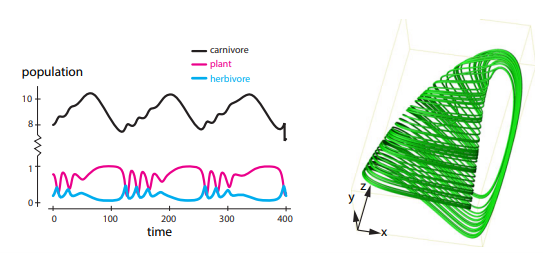
\includegraphics[width=0.7 \textwidth]{Chaos.png}
		\label{Imagen_1}
		\caption{Esquerda: uma simulação do modelo de cadeia alimentar de três espécies descrito no texto com a1 = 5, b1 = 3, a2 = 0,1, b2 = 2, d1 = 0,4, e d2 = 0,01. Direita: uma trajetória típica do modelo de três espécies, Obtido de: \cite{garfinkel_shevtsov_guo_2017}}
	\end{figure}

	\item{Irregularidade}
	
	\par{O comportamento caótico é irregular, ou aperiódico. O comportamento aperiódico nunca se repete exatamente. Se uma trajetória se repetisse exatamente, ou seja, voltasse ao mesmo ponto de estado matemático, ela teria que ser periódica, porque o determinismo exigiria que ele voltasse sempre de novo. Todas as órbitas fechadas são trajetórias periódicas, portanto, os atrativos de ciclo limite são órbitas periódicas fechadas. Sistemas com Os atratores de ponto ou ciclo limite têm transientes iniciais, mas depois se estabelecem em comportamento repetitivo. O comportamento caótico, por outro lado, começa irregular e permanece irregular. Em alguns sistemas, pode parecer que o comportamento se repete e pode se aproximar muito dos valores do estado anterior, mas nunca se repete exatamente  \cite{garfinkel_shevtsov_guo_2017}.}

 
	 \begin{figure}[ht]
	    \centering

		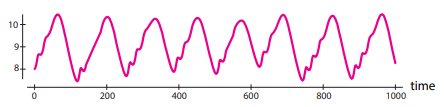
\includegraphics[width=0.7 \textwidth]{Irregularity.png}
		\label{Imagen_2}
		\caption{Série cronológica da população carnívora a partir de uma simulação típica do modelo da cadeia alimentar de três espécies, (Obtido de:  \cite{garfinkel_shevtsov_guo_2017})}
	\end{figure}

 
    \par{ À primeira vista, parece que as populações oscilam, embora de uma forma um tanto complexa. No entanto, um olhar mais atento revela diferenças. A segunda grande oscilação contém uma lomba antes do pico, enquanto a terceira oscilação tem pelo menos duas. Além disso, cada pico tem uma forma um pouco diferente. Esta é a aperiodicidade. Apesar de uma semelhança qualitativa geral, o comportamento do sistema nunca se repete
e nunca se aproxima da repetição. Uma afirmação semelhante é verdadeira sobre a saída do modelo logístico do tempo-discreto. Pode parecer que algumas formas se repetem, mas se olharmos de perto, vemos que a sequência, de fato, nunca se repete.
 \cite{garfinkel_shevtsov_guo_2017}}
    
    \item{Dependência sensível das condições iniciais}
    \par{A característica mais intrigante e famosa do caos é a dependência sensível das condições iniciais. Este termo refere-se ao fato de que em um sistema caótico, duas séries temporais que começam muito próximas uma da outra vão eventualmente se divergir ao ponto o qual seu comportamento é completamente não correlacionado. Em geral, para sistemas multivariados, em tanto o tempo discreto e contínuo, dependências sensíveis significam uma divergência exponencial de trajetórias próximas. existe um número $\lambda$ (greek letter lambda), chamada característica expoente de Lyapunov, a qual:} 
    
    \begin{equation*}
    d ( M_{t} − N_{t} ) = e^{ \lambda  t}  d ( M_{0} − N_{0} )  
    \end{equation*}

    \vspace{0.5 cm}

    \item{Imprevisibilidade}
    
    \par{Talvez você já tenha ouvido falar de Edward Lorenz, o meteorologista e matemático que ajudou a descobrir o caos. Ele fez uma reunião (meeting) chamada "Predicabilidade: a aba das asas de uma borboleta em O Brasil desencadeou um tornado no Texas"... Ele fez uma pergunta: Considere dois planetas que são absolutamente idênticos, até as roupas que você está vestindo hoje, cada árvore, cada detalhe, exceto que no mundo A há mais uma borboleta no Brasil. O que acontecerá com os sistemas meteorológicos dos dois planetas? Talvez você pensou que não haveria diferença em relação a uma mudança tão infinitesimal, mas o bom senso está errado. Na verdade, após pouco tempo, os sistemas meteorológicos irão divergir completamente, para que haja, digamos, um tornado no Texas no mundo A, mas não no mundo B! Dependência sensível das condições iniciais ajudam a explicar uma propriedade fundamental do comportamento caótico, sua imprevisibilidade. \cite{garfinkel_shevtsov_guo_2017}}
    \end{enumerate}
\subsection{Modelos para utilizar}



\subsubsection{Determinista}

\par{O modelo determinístico é um protótipo matemático \cite{Witenberg_1995}, onde as mesmas entradas irão invariavelmente produzir os mesmos resultados, independentemente da consideração da existência do acaso ou da incerteza. Conhecendo com certeza os valores das variáveis, então será assumido que temos todas as informações necessárias para a avaliação de um projeto\cite{ramos_2019}.}

 \subsubsection{Modelo estocástico}

\par{Modelos estocásticos são usados para representar a aleatoriedade e fornecer estimativas dos parâmetros da mídia que determinam o fluxo de fluidos, o transporte de poluentes e a transferência de massa térmica em meios porosos naturais. Este modelo foi desenvolvido pela Ball em 1986, que discutiu que a distribuição de um período infeccioso é permitida para ter qualquer tipo de distribuição que possa ser descrita por sua transformada Laplace. Os modelos estocásticos são construídos em torno de gráficos aleatórios. O processo estocástico é o estudo de como uma variável aleatória evolui ao longo do tempo. Uma variável que não é conhecida antes de um determinado tempo t é chamada de variável aleatória. Se o estado da variável aleatória é conhecido antes de um tempo finito, é chamado de processo estocástico discreto. O processo Markov em cadeia é o melhor exemplo de um modelo estocástico onde a distribuição de probabilidade de tempo t + 1 depende do estado no tempo t e não depende dos estados antes do tempo t \cite{stochastic_model_overview_sciencedirect} \cite{statistical_models_2003}.}
    %% añadir imagen cadena markov

% !!! COMENTARIO aquí no tenemos ninguna cita?
\subsubsection{Modelo Monte Carlo}

    \par{É uma técnica matemática utilizada para estimar os possíveis resultados de um evento incerto. O Monte O método Carlo foi inventado por John von Neumann e Stanislaw Ulam durante a Segunda Guerra Mundial para melhorar a tomada de decisão sob condições de incerteza. Seu nome vem de um cassino bem conhecido em Mônaco, já que o elemento do acaso está no centro da abordagem de modelagem, semelhante a um jogo de roleta. As simulações de Monte Carlo avaliaram o impacto do risco em muitos cenários da vida real, incluindo inteligência artificial, preços de estoque, previsão de vendas, gerenciamento de projetos e preços. Elas também fornecem um número de benefícios para modelos preditivos com entradas fixas, tais como a capacidade de realizar análises de sensibilidade A análise de sensibilidade permite que os tomadores de decisão vejam o impacto de entradas individuais em um determinado resultado, e a correlação permite que eles entendam as relações entre as entradas variáveis \cite{garfinkel_shevtsov_guo_2017}.}
  

\subsubsection{Optimisation}
    \par{Muitos esforços têm sido feitos para descrever situações humanas e sociais complexas. Isto deve ser escrito em uma expressão matemática contendo uma ou mais variáveis, seus valores devem ser determinados. A questão que é formulada, em termos gerais, é para quais valores essas variáveis devem ter um expressão que tem o maior valor numérico possível (maximização) ou o menor valor numérico possível (minimização). Este processo geral de maximização ou minimização é chamado de otimização. Otimização é usada para encontrar a resposta que fornece o melhor resultado, aquela que atinge o maior valor numérico possível.
lucros, produção ou felicidade, ou aquele que atinge o menor custo, desperdício ou desconforto. Com freqüência, estes problemas envolvem o uso mais eficiente de recursos, tais como dinheiro, tempo, maquinaria, pessoal, inventário, etc. problemas de otimização geralmente são classificados como lineares e não lineares, dependendo se as relações do problema respeitam as variáveis.
\cite{Arsham_1996}}

    
    % !!! COMENTARIO aquí no tenemos ninguna cita?
  %%Complex       
    \subsubsection{Complexo}
    \par{Um modelo complexo constitui a descrição matemática de um objeto complexo, aquele que consiste em elementos componentes inter-relacionados, que também podem ser constituídos por seus próprios elementos inter-relacionados. Também, o objeto complexo e seus elementos têm funções e também podem ser decompostos no tempo, porque no caso geral, é necessário tomar decisões relacionadas com o sistema em diferentes períodos. No sistema e em seus elementos atuam interferências do mundo ao redor. Enquanto mais completo será a organização do sistema, menores serão as interferências, mas maior será a complexidade da conciliação de sua operação  \cite{garfinkel_shevtsov_guo_2017}.}
    \par{A diferença entre as palavras complexo e complicado é a seguinte:
    \begin{itemize}
        \item Complicado é algo que consiste em muitas partes ou detalhes diferentes e, portanto, difícil de entender, mas você pode resolver um problema "complicado" analisando separadamente as diferentes partes.
        \item Complexo derivado do latim cum (muitos) plexus (particípio passado "complecti" que significa apertado, abraçado. Portanto, uma situação complexa, um sistema complexo ou um problema resultou da união de várias partes ou elementos, tornaram-se inseparáveis.
    \end{itemize}}
    
    \subsubsection{Caótico}
    \par{O conceito de caos é uma das principais descobertas dos últimos tempos. O caos é observado no dia-a-dia da vida, nas áreas de metrologia, fluxo de fluidos (turbulência), cardiologia, biologia populacional, mercado de ações, modelagem econômica, e assim por diante. As previsões são possíveis em muitos sistemas. Por exemplo, os eclipses podem ser previstos com milhares de anos de antecedência. O movimento de um simples pêndulo (sob hipóteses adequadas), que é governada por uma equação diferencial, é previsível e uma solução de forma fechada pode ser escrita. Entretanto, há muitos fenômenos naturais que não são previsíveis, tais como as previsões meteorológicas, o rolo de dados, e assim por diante, apesar de obedecerem às mesmas leis da física. Acredita-se até recentemente que a previsibilidade pode ser alcançada tendo mais informações e processando-as. Alguns sistemas são "caóticos". - extremamente sensível a pequenas perturbações e imprevisíveis a longo prazo, mostrando o chamado "efeito borboleta". Um sistema complexo também pode ser dependente do caminho, ou seja, seu estado futuro não depende somente de seu estado atual, mas também em sua história passada. \cite{garfinkel_shevtsov_guo_2017}}
    
    
    
     
  
   
    
\newpage

\section{Ferramentas computacionais em modelagem}

\par{A fim de construir um modelo matemático, primeiro é necessário selecionar a estrutura que gostaríamos que fosse equações diferenciais a ter. Em seguida, as equações diferenciais parciais se transformarão em um sistema que  tem um número finito de graus de liberdade. O que significa que o sistema depende de um número definido  de variáveis e parâmetros.}


\par{Normalmente, uma equação simples tem apenas uma desconhecida, e um sistema de três variáveis tem três incógnitas. Mas em sistemas reais de modelagem, é necessário transformar as equações diferenciais em sistemas de equações com muitas incógnitas, empregando métodos numéricos  \cite{garfinkel_shevtsov_guo_2017}.}

\par{A modelagem matemática é feita antes da formulação de qualquer ideia de computador. Nós pegaríamos a onda equação como um exemplo:}

\begin{equation}
    \frac{\partial^2 y}{{\partial x}^2}=\frac{1}{\nu^2} \frac{\partial^2 y}{{\partial t}^2}
\end{equation}

\par{A equação de onda regula ou regra o comportamento do som. Isso é possível de resolver à mão se você assumir que todo o espaço era homogêneo. }

\begin{equation*}
    y= A \cos{ \left( k x - \omega t - \phi \right) }
\end{equation*}

\par{Com:}

\begin{equation*}
    \nu = \frac{ \omega }{ k }
\end{equation*}

\par{Graças a esta equação, a velocidade teórica do som foi descoberta, e sua aproximação foi extremamente próxima ao experimental. No entanto, alguns problemas matemáticos só podem ser resolvidos por um computador, como o som se movendo em um meio heterogêneo  \cite{garfinkel_shevtsov_guo_2017}.}

\par{Utilizando métodos numéricos, podemos encontrar suas soluções dadas por aproximações. Elas implicam operações diversas, como adicionar, subtrair, dividir e derivar, entre outras, que permitem reduzir a complexidade de uma equação, mas aumentar o número de algoritmos de solução  \cite{garfinkel_shevtsov_guo_2017}.}



%PARTE 2.1
    \subsection{Programming languages}
    
    \par{As linguagens de programação são uma ferramenta que pode ser implementada para desenvolver programas de computador (software). Elas podem ser empregadas para projetar e executar instruções para controlar o comportamento físico (hardware), bem como, dispositivos lógicos do computador [Monterde, 2020]. Eles são compostos de uma série de componentes sintáticos que fornecem estrutura e dão sentido a seus elementos e expressões  \cite{garfinkel_shevtsov_guo_2017}.} 
    
     \par{Por outro lado, a programação é o processo de análise, projeto, implementação, testes, e depuração de um algoritmo, sem estes elementos o computador não será capaz de realizar a tarefa desejado pelo usuário  \cite{garfinkel_shevtsov_guo_2017}.} 

    \par{A principal função das linguagens de programação é escrever programas capazes de estabelecer a comunicação usuário-máquina. Para fazer isso, os programas transformam as instruções escritas em código fonte, significado, instruções escritas em linguagem de máquina ou código binário (0 e 1). Quanto aos compiladores, eles traduzem os símbolos de uma linguagem de programação para seu equivalente escrito em linguagem de máquina, este processo é conhecido como compilação (Veja. Figura 3). Finalmente, um programa executável é obtido  \cite{garfinkel_shevtsov_guo_2017}.}
   
    %Imagen 1
	\begin{SCfigure}[0.7][ht]
	    \centering
		\caption{O que é um compilador?, (Obtido de: \href{https://codeforwin.org/2017/05/compiler-and-its-need.html}{Code Forwin})}
		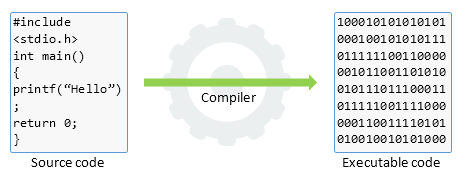
\includegraphics[width=0.7\textwidth]{compiler}
		\label{Fig-Compiler}
	\end{SCfigure}


%Antecedentes
\textbf{Background}

\par{Em meados do século 19, Charles Babbage, professor de matemática e inventor na Universidade de Cambridge, Inglaterra, foi a primeira pessoa a conceber a ideia de uma linguagem de programação. Ada Lovelace é considerado o primeiro programador da história. Ela escreveu o primeiro programa para a máquina previsto por Babbage em cartões perfurados, seguindo a lógica de programação. O que é muito semelhante ao que usamos, no entanto, esses programas nunca puderam funcionar porque a máquina não tinha sido construída  \cite{garfinkel_shevtsov_guo_2017}.} 
\vspace{0.5 cm}
	
	
\par{Em 1823, o governo britânico aprovou o projeto de construir um motor diferente projetado para realizar adições repetidas. Babbage abandonou o projeto para buscar um Motor Analítico, influenciado pelo criação de um fabricante francês de tecidos, Joseph Marie Jacquard, que tinha desenvolvido uma máquina capaz de ler informações codificadas em cartões perfurados de papelão duro (uma folha de papelão que contém informações sob a forma de perfurações de acordo com um código binário). Desde então, a Babbage decidiu construir uma máquina que faria cálculos precisos usando 20 dígitos. Que poderia ser programada usando cartões perfurados  \cite{garfinkel_shevtsov_guo_2017}.} 

%Imagen 2
\begin{SCfigure}[0.5][ht]
	    \centering
		\caption{Punch card, (Obtido de: \href{https://mujeresconciencia.com/2018/06/27/tarjetas-para-programar-el-mundo/}{Women with science})}
		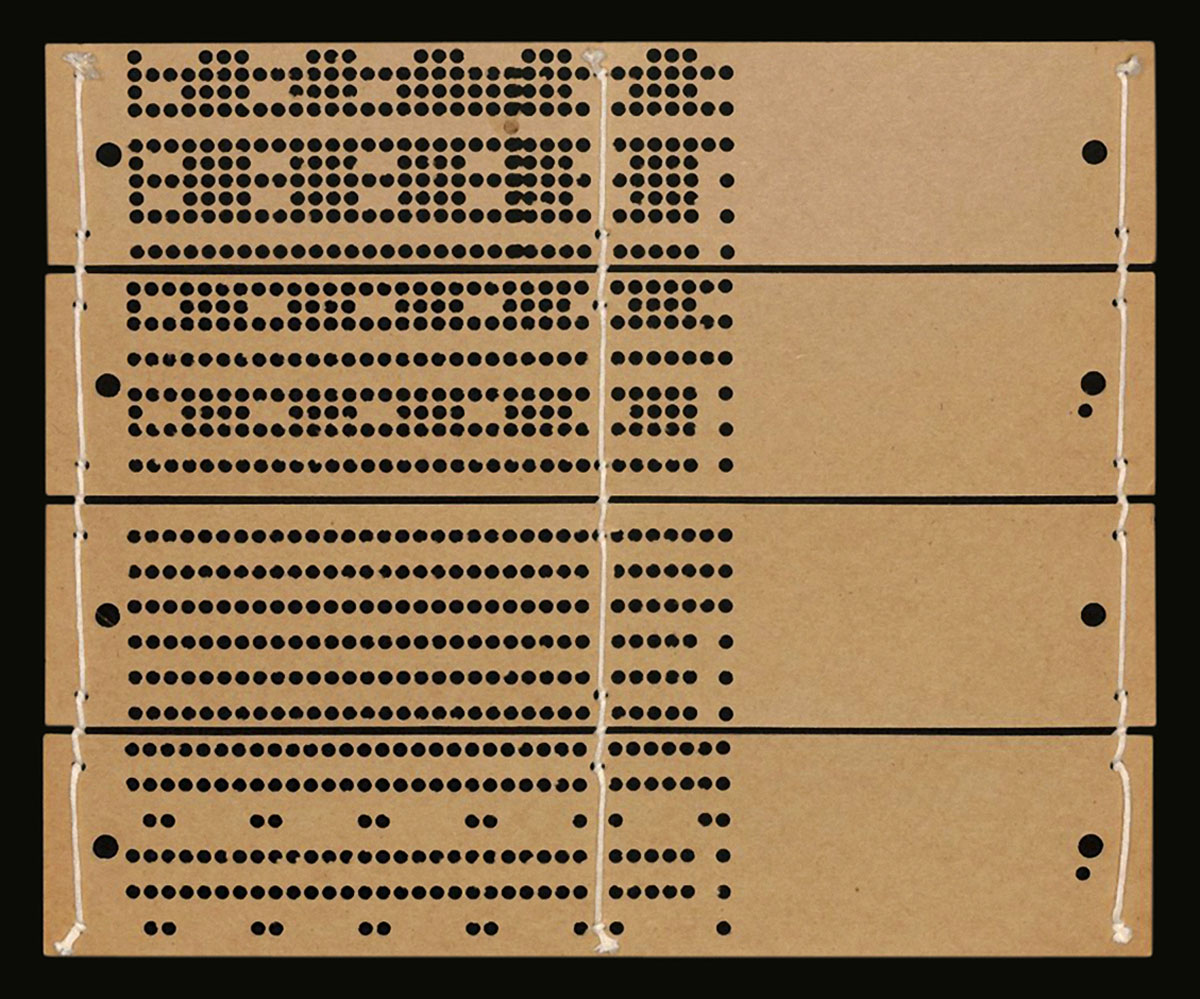
\includegraphics[width=0.5 \textwidth]{Tarjeta.jpg}
		\label{Fig-Perforada}
\end{SCfigure}

\par{Embora esta ideia tenha permanecido apenas no projeto, foi uma contribuição significativa para o projeto e operação dos computadores de hoje. Charles Babbage é considerado o pai da computação. Embora a máquina foi uma inspiração, suas ideias e design serviram para construir e avançar os primeiros computadores modernos  \cite{garfinkel_shevtsov_guo_2017}.}

\vspace{0.5 cm}

%Clasificación
   \textbf{Classificação}
   \par{Os circuitos microprogramáveis são sistemas digitais, que funcionam com dois níveis de tensão simbolizados por zero (0) e um (1). A classificação dos tipos de linguagem é mostrada abaixo:}
   
   \begin{itemize}
       \item{Linguagem de programação de baixo nível: Ela fornece pouca ou nenhuma abstração do microprocessador de um computador, referente ao código binário. Como é orientado para o hardware, ele funciona como instruções para o e com ele é possível construir sistemas operacionais e núcleos.}
        \item{Linguagem de programação de alto nível: Ela se distingue por sua estrutura semântica, que permite que os algoritmos sejam codificados de forma mais natural.}
   \end{itemize} 
   
  
   %Tabla de ejemplos
    \begin{table}[ht]
        \centering
        \resizebox{4.5 cm}{!} {
        \begin{tabular}{| c | c |}
            \hline
            Nível baixo  & Nível alto \\ \hline
            Assembler   & C++ \\
            LOAD X      & Fortran \\
            ADD Y       & Java \\
            STORE Z     & PHP \\
            -           & Python \\
            -           & Perl \\ \hline
        \end{tabular}}
        \caption{Examples}
   \end{table}
   
   
    %Programming Types
   \textbf{Tipos de programação}
   \begin{itemize}
       \item{\textbf{Programação lógica:} É caracterizada pela programação com relações e inferências. Aqui o programador é responsável por especificar as relações lógicas básicas.}
       \item{\textbf{Programação funcional:}É caracterizada pela programação com valores, funções e formas funcionais (que são uma relação entre uma variável dependente e uma variável explicativa). "Um programa funcional consiste em uma expressão, chamemos-lhe E, que está sujeita a regras escritas. A redução consiste na substituição de alguma parte P de E por outra expressão P', de acordo com a regras, este processo é repetido várias vezes até que a expressão resultante não tenha partes que tenham de ser reescritas. A expressão obtida a partir deste processo, E', é o que será a forma normal de E e é o resultado do programa funcional". -H.P. Barendregt.}
       \item{\textbf{Programação Imperativa:} Caracteriza-se por programação com um estado e comandos que modificam esse estado. Temos duas partes importantes: o imperativo, que é uma ordem ou comando, e o procedimento, o ato, o método de proceder, ou uma forma de fazer algo. Quando a programação imperativa é combinada com outros subprogramas é chamada programação processual  \cite{garfinkel_shevtsov_guo_2017}.}
      \item{\textbf{Programação concorrente:} é caracterizada pela programação com mais de um processo. Este tipo de programação é usado para compilar o projeto, alguns problemas são resolvidos de uma forma natural usando um conjunto de processos que operam ao mesmo tempo, uma solução sequencial que se baseia em especificações e reduz o tempo de execução. Há uma diferença entre operações sequenciais e simultâneas. Seqüenciais ocorrem uma após a outra enquanto simultâneas são quando ocorrem ao mesmo tempo.  \cite{garfinkel_shevtsov_guo_2017}.} \item{\textbf{Programação Orientada a Objetos:} Este tipo de programação é caracterizado pela programação com objetos, mensagens e hierarquias de objetos. Enfoca elementos de dados passivos definidos por relações ou atua sobre funções e processos para elementos ativos com seu ambiente  \cite{garfinkel_shevtsov_guo_2017}.} \end{itemize} 
      %Programming languages 
      \textbf{Algumas linguagens de programação} 
      \begin{itemize} 
      \item{ \textbf{C:} Os grandes programas são divididos em pequenos programas chamados funções que são focados em funções e processos que operam com dados. É utilizado em tecnologia da informação, engenharia, gerenciamento, saúde, processamento de imagens e programação de jogos. } 
      \item{\textbf{C\#:} é uma linguagem de programação multiparadigma com fortes disciplinas de programação, escrita, imperativo, declarativo, funcional e orientado a objetos. É utilizado em tecnologia da informação, engenharia, design e controle de qualidade.} 
      \item{\textbf{C++:} é uma linguagem orientada a objetos, é uma linguagem de nível médio, e é uma extensão do Idioma C. É utilizada em tecnologia da informação, informação, engenharia, design, controle de qualidade, administração, software e drivers de firmware. } 
      \item{\textbf{Python:} é uma linguagem interpretada, orientada a objetos e construída sobre uma semântica flexível e robusta. É utilizada em desenvolvimento back-end, tecnologia da informação, engenharia, design, desenvolvimento de web, frameworks, gerenciamento avançado de conteúdo, computação científica e numérica, e gráficos de desktop.} 
      \item{\textbf{Ruby:} é uma linguagem de script de código aberto, orientada a objetos, que pode ser usada isoladamente ou como parte do web framework Ruby on Rails. Ele é usado no desenvolvimento, engenharia de software, engenharia de ciência de dados, desenvolvimento de WebApp, robótica, redes, administração de sistemas e segurança.} 
      \item{\textbf{PHP:}  é uma linguagem de script de código aberto projetada para criar páginas na web dinâmicas que funcionam efetivamente com bancos de dados. Também é usada como uma linguagem de programação de propósito geral. É utilizada para tecnologia da informação, engenharia, design, assistência médica, finanças, administração, aplicação web. desenvolvimento, e roteiros.} 
      \item{\textbf{Java:} é uma linguagem de programação de alto nível, orientada ao usuário, objetos e propósito geral com várias características que o tornam ideal para o desenvolvimento na web. É utilizado em comunicação, educação, finanças, ciências da vida, varejo e serviços públicos, a Internet das Coisas, a nuvem, videogames e aplicativos de celular.}
      \item{\textbf{JavaScript:} é uma linguagem de programação do lado do cliente que roda dentro de um navegador e processa comandos em um computador ao invés de um servidor. Normalmente é colocado em um arquivo HTML ou ASP. Ele é utilizado em Tecnologia da Informação, Engenharia, Design, Marketing, Finanças, Saúde, Front-End Desenvolvimento, e Desenvolvimento de Jogos. Java e JavaScript não estão relacionados.} 
      \end{itemize} 
   %%%%%%%%%%%%%%%%%%%%%%%%%%%%%%%%

   
\subsection{O poder computacional e sua importância}
    
\par{Os supercomputadores são máquinas de computação massivas utilizadas para realizar cálculos complexos em uma grande variedade de aplicações científicas. Tais aplicações abrangem uma ampla gama de tarefas de computação intensiva, incluindo mecânica quântica, previsão do tempo, pesquisa climática, exploração de petróleo e gás, dinâmica molecular e simulações físicas, e requerem uma quantidade de potência e recursos computacionais que vão além do que está disponível em servidores ou estações de trabalho de uso geral \cite{}(R. Gioiosand a 2017). Estes supercomputadores são classificados de acordo com seu desempenho baseando-se em operações de ponto flutuante por segundo (FLOPS). Várias características de medição indicam principalmente o número de operações deste tipo que o processador de hardware pode resolver em um segundo, misturando números pequenos, grandes e até fracionários. (McDonell, 2013)} 

\par{Esta abordagem era muito cara e limitava o uso de supercomputadores em alguns poucos centros de pesquisa em todo o mundo. Para reduzir os custos de aquisição e operação, os pesquisadores começaram a construir supercomputadores a partir de componentes "common off-the-shelf" (COTS), como os utilizados em desktops e laptops de uso geral. Cada supercomputador apresenta um ou mais chips processadores multi-núcleo/multithreaded, vários módulos de memória, um/dois adaptadores de rede, e, possivelmente, alguns discos de armazenamento locais. Mais recentemente, os aceleradores, na forma de unidades vetoriais gráficas ou matrizes de portas de campo programáveis (FPGA), também fizeram seu caminho para a supercomputação convencional. }

\par{Por outro lado, os componentes COTS trouxeram um novo conjunto de problemas que faz com que as aplicações de computação de alto desempenho (HPC) sejam executadas em um ambiente hostil:}
\begin{itemize}
    \item Os componentes COTS são intrinsecamente mais vulneráveis do que os componentes para fins especiais e, por razões computacionais, seguem processos de produção e caminhos de verificação diferentes dos sistemas integrados militares ou de missão crítica da indústria ou mainframes de servidores.
    \item Os componentes COTS não são projetados especificamente para resolver aplicações científicas e seu desempenho de um único processador foi inferior ao processo vetorial, portanto, um número maior de processadores são geralmente necessários para atingir o desempenho desejado. A combinação de um número extremamente grande de componentes do sistema aumenta enormemente a probabilidade combinada de que pelo menos uma interrupção experimente um erro suave, ou deixe de funcionar completa ou parcialmente.
    \item As cargas de trabalho de HPC têm demonstrado ser extremamente heterogêneas e podem possivelmente enfatizar diferentes partes dos supercomputadores, tais como memória, processadores ou rede. Este comportamento heterogêneo, por sua vez, aumenta a tensão térmica e mecânica, reduzindo efetivamente a vida útil de cada um deles. O gabinete e a instalação onde o supercomputador é instalado desempenham um papel importante na resiliência do sistema. Por exemplo, estudos recentes confirmam que o supercomputador instalado em altitudes mais elevadas, como o Cielo no Laboratório Nacional de Los Alamos (LANL), está mais exposto à radiação e apresenta maiores taxas de erro suave.
    \item O simples tamanho dos supercomputadores atuais torna impossível empregar soluções de resiliência comumente usadas em outros domínios, tanto por razões de custo como por razões práticas. As técnicas tradicionais de resiliência, tais como redundância de módulos duplos ou triplos (DMR, TMR), são proibitivas de alto desempenho ou grandes supercomputadores, devido ao grande número de nós de computação e componentes dos nós de computação. 
\end{itemize}

\par {Abaixo estão os 10 melhores supercomputadores:}
\begin{enumerate}[1.]
    \item Supercomputer Fugaku
    %\itprocessesit
    \item Supercomputador Sierra
    \item Sunway TaihuLight
    \item Perlmutter
    \item Selene
    \item Tianhe-2A
    \item is not specifically designed
    \item HPC5
    \item Frontera
\end{enumerate}




\newpage

\section{Ferramentas de bioinformática}
\par{Atualmente existe um grande número de ferramentas que podem facilitar o desenvolvimento da modelagem de sistemas. Esta seção mostra algumas ferramentas que podem ser úteis na modelagem de sistemas biológicos e pequenos exemplos de como elas podem ser aplicadas.}

    \subsection{Cello}
    \par{O cello é uma ferramenta que permite o projeto racional de um circuito genético que fornece um sinal anexo a partir de uma série de dados de entrada. O cello projeta automaticamente uma sequência de DNA que codifica o sinal de saída desejado através das especificações do sensor, como atuadores e restrições de arquivo do usuário. Tudo isso define o organismo e valida as condições de operação. Para estas, é usado a linguagem de hardware Verilog, que cria um diagrama do circuito, atribui portas, alcança um equilíbrio de níveis restritivos quando o modelo de DNA é criado, e simula o rendimento. Como resultado, uma sequência com sistemas booleanos dos organismos requeridos é fornecida e é uma melhor previsão que pode ser feita.}
    \par{Em 2016, a equipe da EPFL utilizou este software. Em seu Frontera, é encontrado o modo como o utilizaram e algumas dicas no caso de outras equipes estarem procurando informações sobre como ele funciona. Eles fornecem informações sobre como utilizá-lo sem conhecer a linguagem de programação Verilog.}
    \par{Para mais informações, clique  \href{https://2016.igem.org/Team:EPFL/Software_CELLO}{aqui}}
    
    \subsection{MATLAB}
    \par{MATLAB é uma plataforma de programação para a solução de problemas computacionais e matemáticos. Esta ferramenta é um ambiente confortável envolvendo computação, visualização e programação, onde é possível expressar os problemas e suas soluções de uma forma matemática [Gilat, 2017]. Alguns dos usos mais comuns do MATLAB são:}
    \begin{itemize}
        \item Cálculo matemático
        \item Criação de algorítmo.
        \item Análise de dados
        \item Criações gráficas
        \item Sistema de modelagem
    \end{itemize} 
    \par{Uma das principais vantagens do uso do MATLAB é que é relativamente fácil de usar e há recursos para aprender de usos simples a mais especializados \cite{Kirouac2019}. Na página \href{https://la.mteensrks.com/support/learn-with-matlab-tutorials,.html}{MathWorks}  você pode encontrar uma variedade de cursos gratuitos e interativos para aprender a usar o MATLAB.}
    \par{Além disso, o MATLAB tem uma grande variedade de caixas de ferramentas que servem a propósitos específicos e tornam seu trabalho mais fácil. Um exemplo de tais caixas de ferramentas que é muito útil para modelagem de sistemas biológicos é SimBiology \cite{Park2019}}
        \subsubsection{SimBiology}
        \par{Esta caixa de ferramentas permite a modelagem, simulação e análise de diferentes sistemas biológicos \cite{Kirouac2019}. SimBiology facilita a criação de equações que descrevem o comportamento de um sistema biológico, fornecendo um ambiente gráfico onde é possível construir um diagrama do sistema e definir parâmetros e tipos de balanços de materiais \cite{Feigelman2016}.}
        \par{SimBiology possui uma grande variedade de facilidades para modelagem de fenômenos biológicos, esta ferramenta possui uma ampla gama de solucionadores numéricos para simulações estocásticas e determinísticas \cite{Ullah2006}}\\
        \par{\textbf{Exemplo de modelagem SimBiology}}
        \par{Um exemplo passo a passo do modelo é uma ligação f histamina a seu receptor e a concorrência provenientes de anti-histamínicos é mostrado. O exemplo foi desenvolvido com a versão 2020b do MATLAB.}
            \begin{enumerate}[1.]
                \item Abra o ambiente gráfico do SimBiology digitando \textit{Simbiology} na janela de comando.
                \item Crie um novo projeto clicando na opção \textit{Create New Blank Model} e dê um nome para o projeto.
                \item Adicione a espécie (histamina, receptor de histamina e anti-histamínico) e uma reação arrastando os elementos dentro do compartimento.
                \item Junte a espécie à reação com Ctrl + Click (Direcionamento é muito importante).
                \item Definir as concentrações iniciais de cada uma das espécies no painel esquerdo.
                \item Marque a reação como reversível (clique na reação para exibir o painel) no painel direito e defina as constantes de reação. 
                \item Salvar o modelo.
                \item Clique no \textit{Model Analyzer} e na nova janela abra o modelo que já foi construído.
                \item No botão  \textit{Program} selecione \textit{Simulate model}, modifique as características nas quais a simulação irá executar e selecione o botão \textit{Run}.
            \end{enumerate}
            
     \subsection{Ferramentas de modelagem de proteínas}
    
   Muitos dos projetos de biologia sintética envolvem proteínas. A compreensão e a previsão dessas moléculas pode ajudar na compreensão de sistemas mais complexos, pode também fornecer insights para projetar experimentos. Esta é a razão pela qual dedicamos uma seção para mostrar algumas das ferramentas que podem ser úteis na modelagem de proteínas.
        \subsubsection{I-TASSER}
        \par{O I-TASSER é um servidor online que pode ser usado para a visualização das possíveis estruturas na fusão das proteínas, para que possamos ter informações sobre sua função. Sequências de aminoácidos, são usadas como entrada e com elas o servidor busca informações no Banco de Dados de Proteínas e envia modelos de proteínas com dobras similares, com imagens 3D e uma previsão das propriedades da proteína. }\\
        \par{\textbf{Exemplos de I-TASSER}}
        \par{Um exemplo de como utilizar este servidor para o modelo de uma proteína é mostrado abaixo:}
            \begin{enumerate}[1.]
            \item Abra a página do I-TASSER
            \item Na seção Serviços Online selecione a janela do I-TASSER
            \item Digite a seqüência de proteínas no formato FASTA ou selecione um arquivo com a seqüência
            \item Faça o login ou crie uma conta
            \item Atribuir uma identificação para que você possa ter o controle de sua seqüência
            \item Aguarde os resultados

            \end{enumerate}
        \subsubsection{AlphaFold}
            \par{AlphaFold é uma IA que pode prever a estrutura 3D de uma proteína a partir de suas sequências de aminoácidos \cite{Kiersten}. Alphafold prevê sequências através de uma rede neural, que combina alinhamento de sequências e características proteicas homólogas para gerar uma estrutura com maior precisão em comparação a outras ferramentas de predição de proteínas. \cite{DAVID}.}
            \par{Esta ferramenta tornou possível prever a estrutura 3D de todo o proteoma humano \cite{DAVID}.}
            %Actualizar referencias con Bib.
        \subsubsection{Phyre\texorpdfstring{$^2$}{Lg}}
        \par{O Phryre 2 é um motor de reconhecimento de homologia/analogia de proteínas(). É a segunda versão do Phyre original do servidor, com novas atualizações e melhorias em sua precisão e um redesenho mais intuitivo e rápido da interface do servidor().} 
        \par{Esta ferramenta é usada para modelar e prever a estrutura tridimensional (3D) de uma ou várias proteínas usando sequências de proteínas ou genes(). Ela também permite modelar proteínas com base em uma estrutura modelo fornecida pelo usuário, assim como proteínas multidomínio. Para realizar este processo, ele usa o alinhamento oculto do modelo Markov via HHsearch para aumentar a precisão do alinhamento e a taxa de detecção().}  
        
        \par{Ele possui uma biblioteca com informações sobre novas estruturas, códigos PBD e homólogos. Ela também fornece dois modos para modelagem: normal e intensivo().}
            \par{\textbf{Normal:} permite uma determinação rápida mas aproximada da estrutura proteica.}
            \par{\textbf{Intensive:} Permite determinar a estrutura da proteína com mais precisão, mas o processo é lento.}
        \par{\textbf{Benefícios:()}}
        \begin{itemize}
            \item Maior longevidade nos resultados (1 mês).
            \item  Permite visualizar e renovar o trabalho anterior.
            \item Está pronto para publicação.
            \item Criação de gráficos.
            \item Prevê o site de encadernação e a hélice transmembrana.
        \end{itemize}
        \par{\textbf{Extensões:}}
        \par{Phryre 2 apresenta uma simulação ab initio chamada \textbf{Poing}, que serve para modelar seções da proteína sem homologia detectável através de estruturas conhecidas. Para fazer isto, Poing as assimila como molas elásticas lineares e modela as seções com sua simulação física.}
        \par{\textbf{BackPhyre} é o inverso de Phyre, ele não prevê a estrutura 3D de uma sequência, mas com base em a estrutura da proteína que faz uma comparação com uma estrutura relacionada a um genoma de interesse.()}
        \par{\textbf{Phyre Alarm} permite adicionar um sequencímetro e comparar com novas informações adicionadas à biblioteca de curvas (é atualizado semanalmente). Se for encontrado, os resultados são notificados por e-mail()}
        \par{\textbf{Steps to model:}}
            \begin{enumerate}[1.]
            \item Busque em seu navegador Phyre 2. 
            \item Cadastre-se na plataforma.
            \item Confirme seu e-mail.
            \item Preencha os dados necessários no espaço em branco: e-mail e sequência de aminoácidos. \textbf{Dica:} Se você tiver mais de 5 ou 6 sequências para modelar usar a opção "Batch", disponível no modo Expert após o login. 
            \item Modo de seleção: normal ou intensivo.
            \item Selecione o propósito de usar o servidor: sem fins lucrativos, com fins lucrativos ou outros.
            \item Clique em "Phyre Search".
            %\begin{figure}
                   
            %\end{figure}
            \item Espere, o tempo de espera depende da duração de sua sequência.

            \item Os resultados serão enviados por e-mail.
            %\begin{figure}
                   
            %\end{figure}
            \end{enumerate}
        \par{\textbf{Exemplo:}}
        \href{https://2020.igem.org/Team:KCL_UK/Structural_Modelling } 
        
        \subsubsection {PyMOL}
        \par{PyMOL é um sistema de visualização molecular para análise e compartilhamento de dados moleculares baseado no software Python \cite{Yuan_2017} que interpreta mais de 30 formatos de arquivo e até suporta scripts personalizados. Graças a uma nova interface de usuário unificada, é possível criar filmes rapidamente e facilmente através de uma interface molecular, bem como transformar estruturas protéicas com diferentes texturas e trajetórias animadas com vários efeitos de movimento. Da mesma forma, você pode personalizar o gráfico codificando segmentos ou mudando cores das cordas \cite{Schrödinger_2022}}. 
        \par{\textbf{Benefícios(\cite{DeLano_2022}):}}
            \begin{itemize}
                \item Sistema rápido e não pesado.
                 \item Imagens de boa qualidade.
                 \item Inclui fragmentos pré-construídos.

                 \item Personalização.
                 \item Os elementos podem ser ligados ou desligados.
            \end{itemize}
            \par{\textbf{Extensões:}}
            \par{Com \textbf{AxPyMol} dados moleculares interativos podem ser inseridos e visualizados(\cite{PyMOL_2016}).}
            \par{\textbf{Exemplo:}} \href{https://2021.igem.org/Team:ASIJ_Tokyo/Protein_Model}
            
           \subsection{Ferramentas de simulação de interação molecular}
\subsubsection{UCSF Chimera}
        \par O Chimera é um programa multifuncional que permite o acoplamento molecular entre proteínas e pequenos ligandos de arquivos .pdb. Além disso, este programa permite a visualização e análise das estruturas através de mapas de densidade e alimentação de sequências. Além disso, permite a cor das cadeias das proteínas e mostra as interações entre as proteínas-ligantes.

\begin{SCfigure}[0.65][ht]
	    \centering
		\caption{Visualização do complexo de vínculo proteico em Quimera   \cite{Pettersen_2004}}
		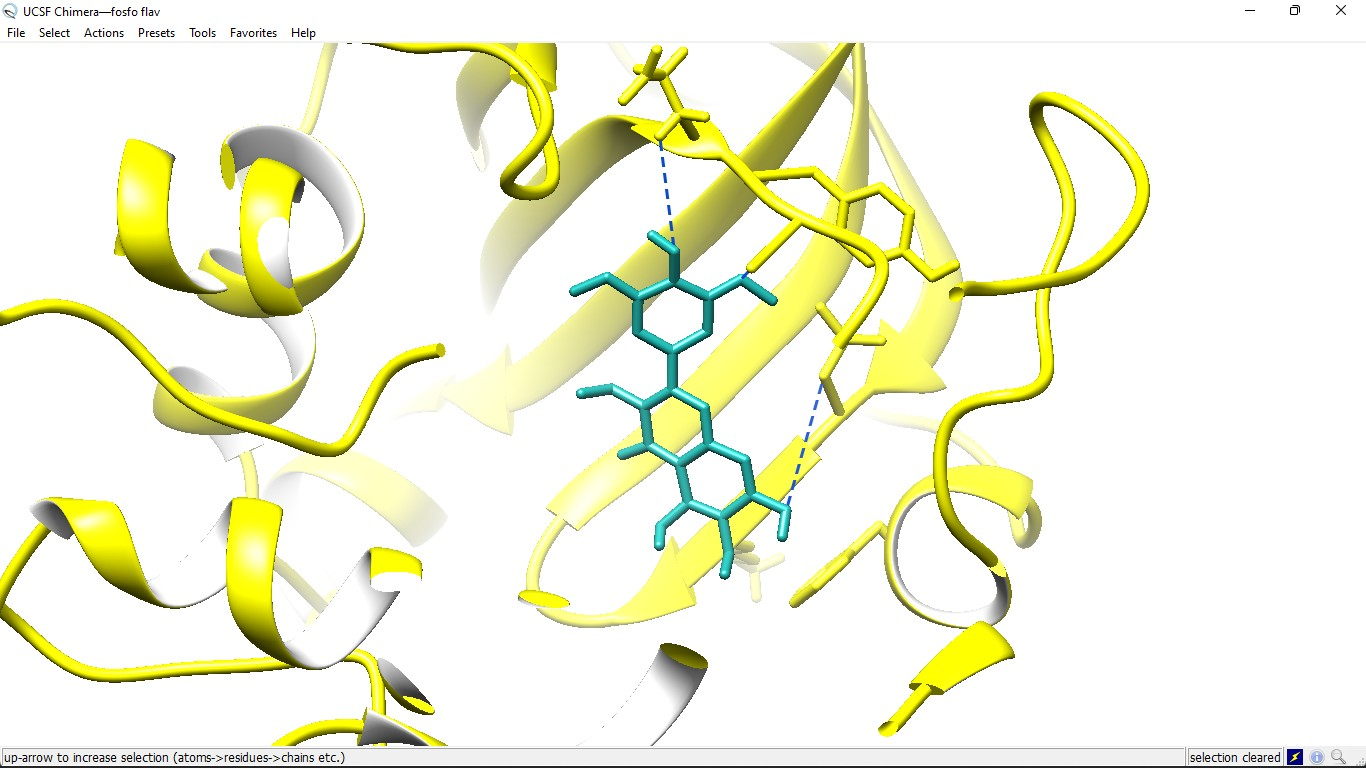
\includegraphics[width=0.65\textwidth]{chimera}
	\end{SCfigure}

        \par{\textbf{Passo a passo}}
        \par{A seguir, apresentamos os passos básicos de como atracar com este programa:}
            \begin{enumerate}[1.]
            \item Uma vez que você tenha suas proteínas e ligantes, abra o programa Chimera USCF.
            \item Em seguida, abra seus arquivos no programa. Será necessário adicionar os estados de protonação e atribuição de cargas.
            \item Salvar os arquivos prévios carregados e protonados com extensão .mol2.
            \item Execute o acoplamento molecular através da AutoDock Vina.
            \item Salve as poses obtidas com a extensão .pdb.
            \end{enumerate} 
\subsubsection{ArgusLab}
        \par ArgusLab é um programa de licença gratuito com uma interface gráfica de fácil utilização. É um visualizador e editor de estruturas biológicas ou moléculas orgânicas, e permite fazer docking molecular. A vantagem do ArgusLab, sobre outros programas de seu tipo, é que ele incorpora parâmetros de campos de força para vários metais como Ni, Cu, Ti, Co, Mn, e mais. Desta forma, a diversidade de Ligantes e Receptores pode ser analisada utilizando estudos de acoplamento molecular.
        
\begin{SCfigure}[0.65][ht]
	    \centering
		\caption{Visualização de ligações protéicas complexas no ArgusLab  \cite{Thompson_2004}}
		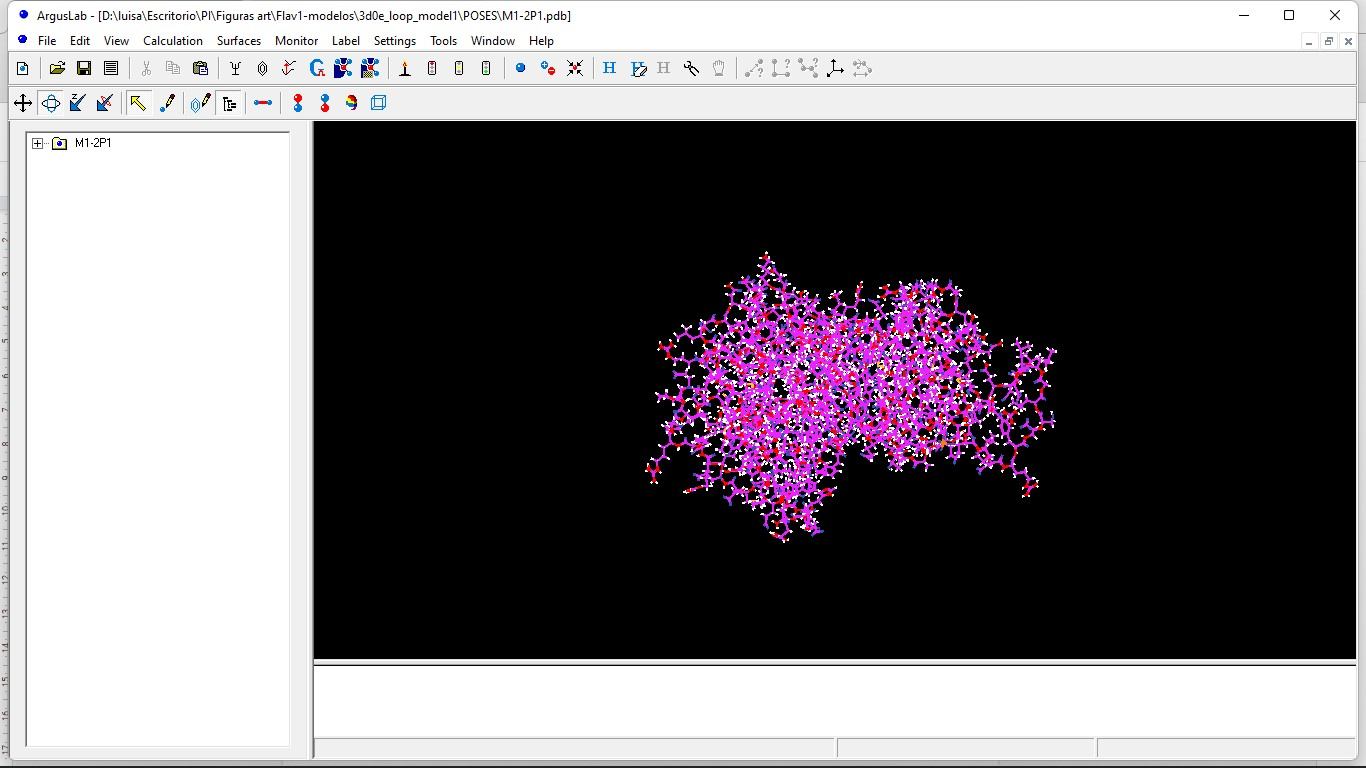
\includegraphics[width=0.65\textwidth]{argus}
	\end{SCfigure}     
	\par{\textbf{Passo a passo}}
        \par{A seguir, apresentamos os passos básicos para considerar como atracar com este programa:}
            \begin{enumerate}[1.]
            \item Uma vez que você tenha suas proteínas e ligantes, abra o programa ArgusLab.
            \item Abra seus arquivos no programa.
            \item Apague as moléculas de água por shift + click na última molécula de água/clique direito/delete.
            \item Selecione os aminoácidos do site de ligação e faça um grupo com eles. Em seguida, faça o mesmo com seu ligan
            \item Execute o acoplamento das moléculas com a opção Calculation/Dock a Ligand.
            \item Salvar os resultados em extensão .pdb.
            \end{enumerate}

        \subsubsection{PyRx}
        \par PyRx é um programa que permite fazer docking molecular entre proteínas e pequenas ligações através da AutoDock Vina. Além disso, você pode ter uma visualização básica das moléculas.
       
\begin{SCfigure}[0.65][ht]
	    \centering
		\caption{Visualização de ligações proteicas complexas em PyRx  \cite{Dallakyan_2014}}
		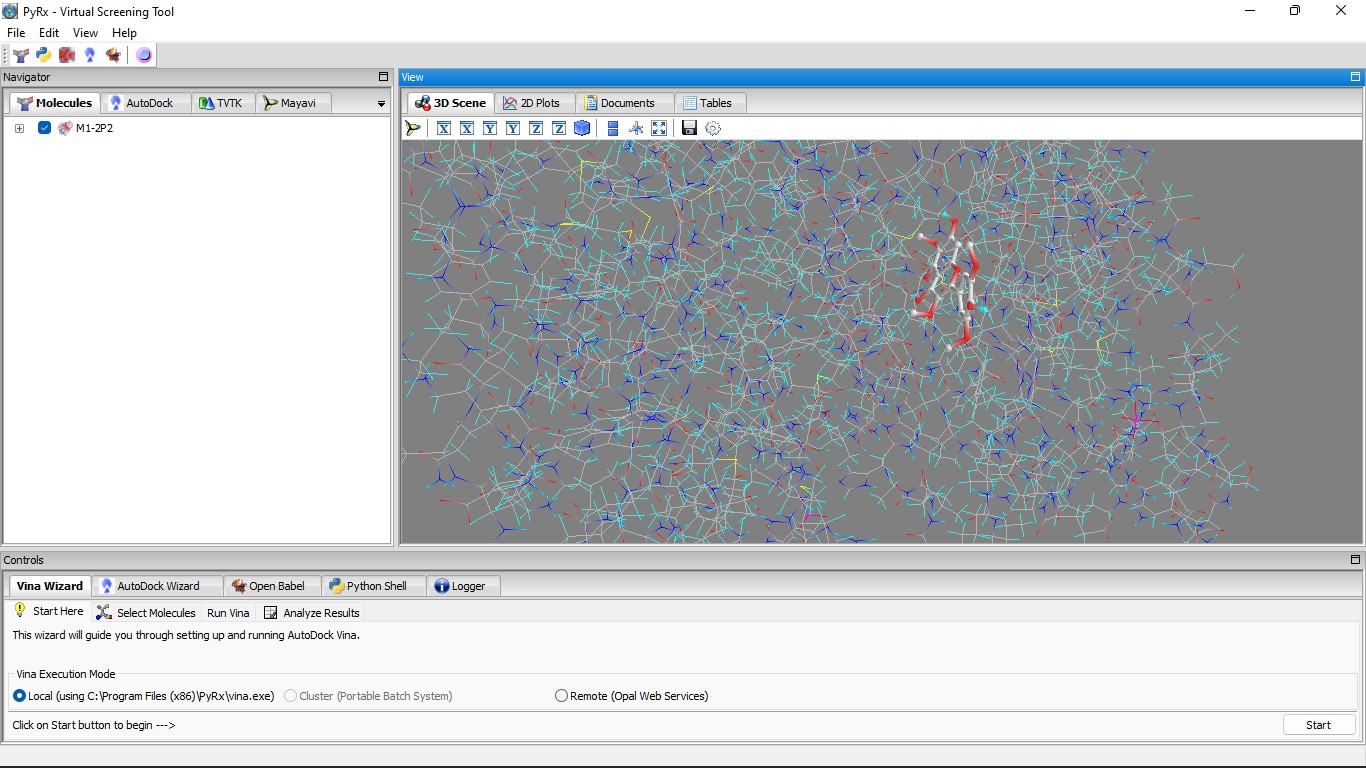
\includegraphics[width=0.65\textwidth]{pyrx.jpg}
	\end{SCfigure}
	
    \par{\textbf{Passo a passo:}}
    \par{A seguir, apresentamos os passos básicos de como atracar com este programa:}
            \begin{enumerate}[1.]
            \item Uma vez que você tenha suas proteínas e ligantes, abra o PyRx.
            \item Abra seus arquivos no programa na seção AutoDock/Vina Wizard.
            \item Defina as condições da caixa de acoplamento molecular.
            \item Execute o docking molecular
            \iteclickve Salvar os resultados em extensão .pdb
            \end{enumerate}

        \subsubsection{Swiss-Model}
        \par Swiss-Model é um servidor de modelagem de estrutura de proteínas totalmente automatizado, acessível através do servidor Expasy, ou do programa DeepView (Swiss Pdb-Viewer). O objetivo deste servidor é fazer modelagem de proteínas acessível a todos os pesquisadores da ciência da vida em todo o mundo.
        
        \par \textbf{Passo a passo:}
            \begin{enumerate}
                \item Seleção do modelo de proteína
                \par  O melhor modelo deve ser selecionado. Os critérios para selecionar a estrutura usada como referência permanecem os mesmos que nos passos do MODELLER. Preste atenção ao valor de identidade ($>$ 25\%) ntre as sequências, melhor cobertura, baixo valor e melhor resolução cristalográfica (quanto menor, melhor).
               \item Alinhamento e construção do modelo
               \par A SWISS-MODEL já trabalha o alinhamento internamente. Você só precisa selecionar o modelo da lista de seleção e o servidor vai buscar o arquivo PDB. O modelo é então construído com base no modelo e no alinhamento após clicar em "Construir Modelos". Podemos ver que o SWISS-MODEL elimina automaticamente a região do peptídeo do sinal e não permite a inserção do peptídeo do sinal.
                \item Avaliação do modelo
                \par A SWISS-MODEL tem suas próprias ferramentas de avaliação. Para avaliar o modelo, deve-se prestar atenção aos valores QMEAN (Qualitative Model Energy Analysis) e GMQE (Global Model Quality Estimation). O QMEAN é um estimador conhecido como z-score. Quando o valor z está próximo de 0, significa que o modelo é considerado confiável e, portanto, há uma boa concordância entre o modelo e estruturas experimentais de tamanho semelhante. As propriedades geométricas fornecem uma estimativa da qualidade global absoluta. O GMQE, por outro lado, está em uma faixa de 0 a 1. Quanto mais alto for, mais preciso será o modelo com relação ao alinhamento e cobertura do modelo alvo. O SWISS-MODEL também fornece um gráfico Ramachandran interativo na página web. A estatística da trama Ramachandran é 96,72$\%$ dos resíduos em regiões favoráveis. Após o download do modelo, uma comparação visual entre o modelo e as estruturas do modelo pode ser feita por alinhamento estrutural usando a ferramenta PyMOL.
            \end{enumerate}

\subsubsection{CHARMM-GUI}
        \par Entre várias ferramentas de modelagem baseadas na web, CHARMM-GUI,[http://www.charmm-gui.org], se propõe a simplificar e generalizar os protocolos para construir sistemas complexos de simulação e preparar arquivos de entrada de simulação para pacotes de simulação amplamente utilizados, tais como CHARMM, NAMD, GROMACS, AMBER, GENESIS, LAMMPS, Desmond, OpenMM e CHARMM/OpenMM para facilitar o uso de técnicas avançadas de simulação \cite{Jo_2017}.
     
        
        \par Desde seu desenvolvimento em 2006, CHARMM-GUI expandiu-se para uma gama de capacidades e agora contém vários módulos diferentes projetados para configurar uma ampla gama de sistemas biológicos (Fig. 1) \cite{Jo_2017}.
        
        \par O fluxo de trabalho implementado no servidor HDOCK é mostrado na Figura 8.
        \begin{SCfigure}[0.65][ht]
	    \centering
		\caption{Visão esquemática dos módulos no gerador de entrada CHARMM-GUI. [A figura colorida pode ser vista em willeyonlinelibrary.com]\cite{Jo_2017} )}
		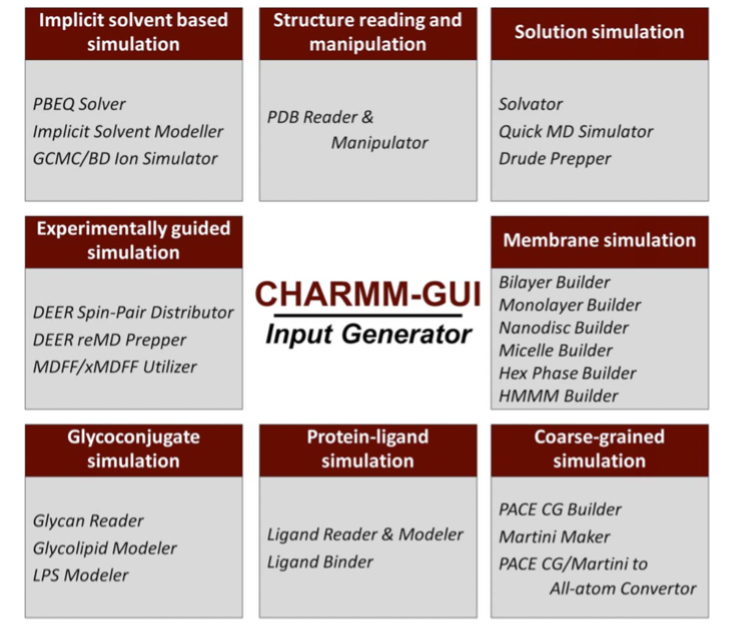
\includegraphics[width=0.65\textwidth]{images/Imagen 1.png}
	\end{SCfigure}\textbf{}
        
        \par A filosofia no desenvolvimento do CHARMM-GUI não se trata tanto de fornecer os elementos essenciais da modelagem molecular, mas também de ajudar os usuários a realizar uma tarefa, como construir um sistema de membrana ou dissolver uma proteína, fornecendo uma interface otimizada que torna o CHARMMGUI acessível aos usuários com menos experiência em ferramentas de modelagem e ainda útil para especialistas, especialmente por gerações de sistemas em lote \cite{Jo_2017}.
        
       \par Uma limitação importante é que o CHARMM-GUI contém muitos parâmetros padrão (por exemplo, o número de etapas para minimização ou os detalhes de como solvatar uma proteína), que são ocultados dos usuários e podem tornar o CHARMM-GUI menos atraente para usuários mais avançados para suas necessidades específicas de customização \cite{Jo_2017}. 

\subsubsection{HDOCK}
		\par {Proteínas e ácidos nucleicos são os dois tipos mais importantes de macromoléculas biológicas na célula. Suas interações são cruciais para muitos processos biológicos, como transdução de sinal, regulação celular, síntese de proteínas, replicação e reparo de DNA, transcrição de RNA, etc. Portanto, a determinação de suas estruturas complexas é valiosa para entender o processo biológico em nível atômico e, assim, desenvolver intervenções terapêuticas ou medicamentos direcionados a essas interações. Dado o alto custo e as dificuldades técnicas dos métodos experimentais, o docking molecular, que prevê computacionalmente o complexo a partir de estruturas individuais, vem desempenhando um papel importante na determinação de estruturas complexas \cite{Yan_2017}. Para fazer uso automático das informações de ligação do PDB no dock, o HDOCK é um servidor web muito útil.}
		
   \par {O servidor HDOCK (http://hdock.phys.hust.edu.cn/) é um conjunto altamente integrado de pesquisa de homologia, modelagem baseada em modelos, previsão de estrutura, docking macromolecular, informações biológicas e gerenciamento de tarefas para um docking proteína-proteína robusto e rápido. O servidor HDCOK distingue-se de servidores de docking semelhantes em sua capacidade de suportar sequências de aminoácidos como entrada e uma estratégia de docking híbrida na qual informações experimentais sobre o local de ligação proteína-proteína e espalhamento de raios X de pequeno ângulo podem ser incorporadas durante o docking e os processos de pós-docking. Além disso, o HDOCK também suporta o docking de proteína-RNA/DNA com uma função de pontuação intrínseca. O servidor fornece templates e docking baseados em modelos de ligação de duas moléculas e permite o download de uma visualização interativa. O servidor HDOCK é usuário e processou 30.000 trabalhos de encaixe desde seu lançamento oficial em 2017. O servidor normalmente pode concluir um trabalho de encaixe em 30 minutos \cite{Yan_2020}}

		\par {O fluxo de trabalho implementado no servidor HDOCK é mostrado na Figura 9. }
        \begin{SCfigure}[0.65][ht]
	    \centering
		\caption{O fluxo de trabalho do servidor web HDOCK é dividido em quatro etapas: (1) entrada de dados, (2) busca de similaridade de seqüência, (3) modelagem de estrutura e (4) acoplamento global baseado em FFT, no qual é dada prioridade às estruturas de entrada do usuário. ] \cite{Yan_2017})}
		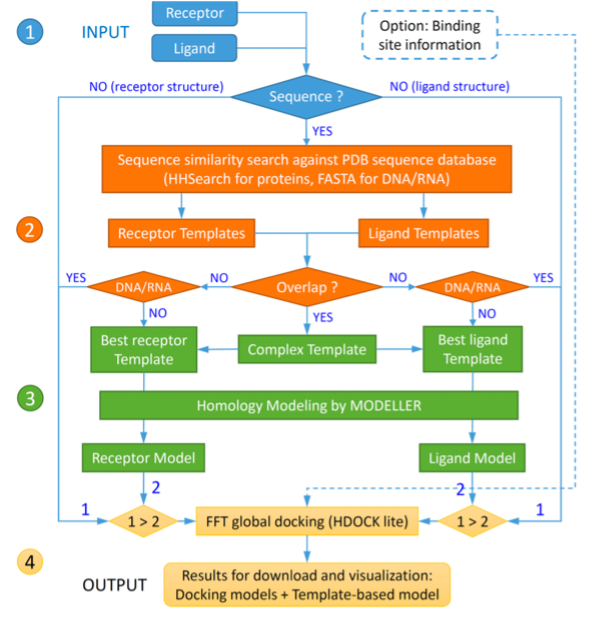
\includegraphics[width=0.65\textwidth]{Imagen 2.png}
	\end{SCfigure}\textbf{}

\par De acordo com \cite{Jo_2017} para melhor facilitar o uso do servidor HDOCK por usuários normais, especialmente para usuários sem experiência, o servidor foi projetado para aceitar tanto entradas de sequência e estrutura para proteínas, duas para estruturas e duas para sequências, como segue:
1)	Faça upload do seu arquivo pdb no formato PDB.
2)	Forneça seu arquivo pdb em PDB ID: ChainID (e. g., 1CG1: E).
3)	Copie e cole sua sequência de proteínas abaixo no formato FASTA.
4)	Carregue seu arquivo de sequência de proteínas no formato FASTA.

\subsubsection{GLYCAM-Web}
Muitas áreas de pesquisa, particularmente aquelas focadas em aspectos estruturais de biomoléculas, “migraram para o ciberespaço” nos últimos 20-30 anos. Este movimento tornou-se ainda mais proeminente nos últimos 5-10 anos, amplificado pela maior acessibilidade ao espaço (de dispositivos móveis para a nuvem) e por recursos cada vez mais sofisticados e poderosos disponíveis para computação de alto desempenho. O campo da glicobiologia estrutural tem se beneficiado muito desse progresso e tem aproveitado as ferramentas e recursos computacionais desenvolvidos especificamente para a análise estrutural de carboidratos \cite{Yuriev_2015}.
O GLYCAM-Web está focado na previsão de estruturas tridimensionais (3D) de carboidratos e estruturas macromoleculares que incluem carboidratos. O servidor é criado e operado pelo grupo de pesquisa do Prof. Robert J. Woods no Centro de Pesquisa de Carboidratos Complexos (CCRC) da Universidade da Geórgia em Atenas. O servidor pode realizar modelagem conformacional de oligossacarídeos, bem como modelagem 3D de glicoproteínas.  
As principais interfaces para modelar conformações de oligossacarídeos são:
1. Carbohydrate Builder [incluindo um Builder especial para glicosaminoglicanos (GAGs)]
2. O  Glycoprotein Builder e as Bibliotecas de Oligossacarídeos.  
3. e as Bibliotecas Oligosaccharide são anexos relevantes para modelar a conformação oligosaccharide. O servidor é de fácil utilização e permite uma gama de opções de upload e download.
Dada uma variedade de formatos de arquivo frequentemente, programas específicos usados em modelagem molecular, facilidade de uso relacionada à portabilidade dos formatos de arquivo é um importante recurso "real-estate" altamente valorizado pelos moradores do ciberespaço \cite{Yuriev_2015}.

    \subsection{Ferramentas de simulação de interações moleculares}
                \subsubsection{GROMACS}
        \par{GROMACS é um programa multiplataforma de código aberto para realizar simulações de dinâmica molecular e minimização de energia de sistemas com centenas de milhões de partículas. Isso permite conhecer e prever o comportamento de propriedades macroscópicas através da descrição de sistemas químicos complexos em termos de um modelo atômico realista.}
        \par{Verificando um pequeno exemplo \cite{Villa_2017}, veremos a visualização de uma pequena proteína (Fator Xa, código PDB:v1FJS), que é uma proteína que gera coágulos sanguíneos.
Para visualização:
}
        \\
        
        \par{import nglview as ng}
        \par{$view = ng.show_structure_file("input/1fjs.pdb")$}
        \par{view}
        \\
        
        \par{Desta forma podemos ver uma imagem como a da Figura 3.}
        \begin{SCfigure}[0.65][ht]
	    \centering
		\caption{Visualização do fator Xa (Fonte: \cite{Villa_2017})}
		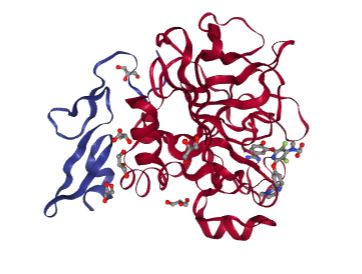
\includegraphics[width=0.65\textwidth]{Proteina.JPG}
	\end{SCfigure}
	
\par{No entanto, esta visualização contém átomos que não correspondem à estrutura da proteína. Para remover esses átomos (chamados "HETATM" no arquivo PDB), basta usar o grep:
}

\vspace{0.5 cm}

\par{$!grep -v HETATM input/1fjs.pdb > 1fjs_protein_tmp.pdb$}
\par{$!grep -v CONECT 1fjs_protein_tmp.pdb > 1fjs_protein.pdb$}
\par{To visualise it:}
\par{Import nglview as ng}
\par{$view = ng.show_structure_file("1fjs_protein.pdb")$}
\par{view}
\\

\par{Assim obtemos uma estrutura mais pura como na Figura XXX:}

\begin{SCfigure}[0.65][ht]
	    \centering
		\caption{Visualização do Fator XA puro (Fonte\cite{Villa_2017})}
		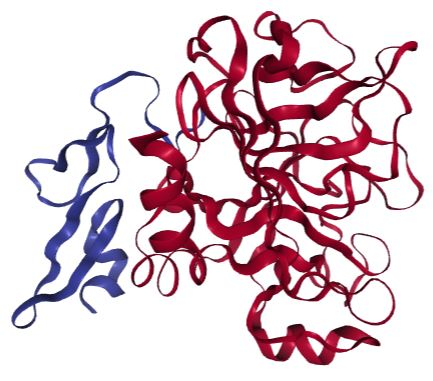
\includegraphics[width=0.5\textwidth]{ProteinaPura.JPG}
	\end{SCfigure}


\subsubsection{AutoDocks}
\par{O Autodock é um dos softwares de simulação de modelos moleculares mais utilizados, projetado para prever a ligação entre pequenas moléculas e receptores com estrutura tridimensional conhecida. Os cálculos realizados são desenvolvidos em 4 etapas principais:}
\vspace{0.4 cm}

\par{Preparação do Arquivo de Coordenadas: Durante este estágio, o ligante e o receptor são preparados para incluir as informações necessárias para usar o AutoDock. Para isso, são utilizados arquivos do tipo PDBQT que incluem átomos de hidrogênio polares, cargas parciais, tipos de átomos e informações sobre a articulação de moléculas flexíveis. Para gerar esses arquivos é possível usar o AutoDockTools}
    \par{Executando o AutoGrid: A execução do AutoDock requer um mapa de grade pré-computado para cada tipo de átomo no ligante passando pelo docking. Esses mapas consistem em uma rede tridimensional de pontos regularmente espaçados ao redor de uma região de interesse na macromolécula em estudo. Para executar o AutoGrid, o seguinte código é usado:}
    
\vspace{0.4 cm}
    autogrid4 -p macro.gpf [-l macro.glg]
\vspace{0.4 cm}

    \par{O docking molecular com AutoDock: AutoDock avalia as interações proteína-ligante em cada ponto usando uma simulação de cluster. Para isso, o AutoDock requer um mapa calculado pelo AutoGrid, um ligante no formato PDBQT e um arquivo de parâmetros para clustering. Os cálculos começam com o seguinte código:}
\vspace{0.4 cm}

autodock4 [-i][-u][-t] -p lig.dpf [-l lig.dlg]

\vspace{0.4 cm}

\par{Avaliação dos resultados: Ao final da simulação, são obtidas as coordenadas de cada ponto onde foi feita a ligação, bem como informações sobre a formação de clusters e energias de interação. O processamento desses dados pode ser feito na seção “Analyse” no menu AutoDockTools.}

\newpage

\subsubsection{ClusPro} %02/10/2022

\par{O servidor ClusPro é utilizado para a análise estrutural de um encaixe proteína-proteína e os resultados obtidos podem permitir a identificação das melhores conformações de encaixe. O ClusPro possui uma interface de usuário básica, mas também permite aplicar várias opções avançadas na busca, como remover regiões de proteínas não estruturadas, aplicar atração ou repulsão, contabilizar restrições de distância de pares, construir homomultímeros e localizar sítios de ligação de heparina (Kozakov et al., 2017). A execução das análises no servidor é realizada seguindo três etapas computacionais (Kozakov et al., 2017):} 

\begin{enumerate}
    \item Encaixe de corpo rígido por amostragem de bilhões de conformações;
    \item Agrupamento baseado no desvio quadrático médio (RMSD) das 1.000 estruturas de menor energia geradas, para encontrar os maiores agrupamentos que representarão os modelos mais prováveis ​​do complexo;
    \item Refinamento de estruturas selecionadas usando minimização de energia.
\end{enumerate}

\subsubsection{PIPER}

\par{O PIPER é um programa de ajuste baseado na abordagem de correlação Fast Fourier Transform (FFT) e é usado na etapa de ajuste de corpo rígido. Uma proteína receptora é colocada na origem do sistema de coordenadas em uma grade fixa, enquanto uma proteína ligante é colocada em uma grade móvel. Nesse processo, a energia de interação é escrita na forma de uma função de correlação e o algoritmo baseado em FFT permite o ajuste de proteínas sem informações prévias sobre a estrutura do complexo (Kozakov et al., 2017).}

\subsubsection{PatchDock}

\par{PatchDock emprega uma técnica semelhante à um quebra-cabeças. Dadas duas moléculas, suas superfícies são divididas em pedaços de acordo com a forma da superfície. Estes pedaços correspondem a padrões que se distinguem visualmente. Uma vez identificados os pedaços, eles podem ser sobrepostos usando algoritmos de formas correspondentes. O algoritmo possui três estágios principais:}

\begin{enumerate}
    \item Representação da Forma Molecular - nesta etapa, a superfície molecular da molécula é calculada. Depois, é aplicado um algoritmo de segmentação para detecção de manchas geométricas (peças côncavas, convexas e de superfície plana). Os pedaços são filtrados, de modo que somente pedaços com resíduos de "hot spot" são retidos.
    \item Correspondência de Pedaços de Superfície - um híbrido das técnicas de correspondência de Geometric Hashing e Pose-Clustering é aplicado para corresponder aos pedaços detectados na etapa anterior. Os pedaços côncavos são combinados com pedaços convexos e planos com qualquer tipo de pedaços.
    \item Filtragem e Pontuação - os complexos candidatos da etapa anterior são examinados. Todos os complexos com penetrações inaceitáveis dos átomos do receptor para os átomos do ligante são descartados. Finalmente, os candidatos remanescentes são classificados de acordo com uma pontuação de complementaridade de forma geométrica.

\end{enumerate}

\par{Os resultados do PatchDock são apresentados em uma lista com os complexos receptor-ligante candidatos. A lista é apresentada ao usuário no formato de uma tabela, cada linha de tabela representa um complexo de candidatos. Os parâmetro utilizados são:}

\par{Os parâmetros usados são:}
\begin{itemize}
    \item\textbf{ Solution No:} Número do complexo candidato

    \item \textbf{Score:} Pontuação de complementaridade de forma geométrica. Os complexos candidatos são ordenados de acordo com esta pontuação.

    \item \textbf{Area:} Área aproximada de interface do complexo.

    \item\textbf{ACE:} Energia de contato atômica

    \item \textbf{Transformation 3D:} 3 ângulos de rotação e 3 parâmetros translacionais. A transformação é aplicada sobre a molécula ligante.

    \item \textbf{PDB file of the complex:} A estrutura complexa prevista no formato PDB.

\end{itemize}

\subsubsection{FireDock}

\par{Como mais um software para análise e pontuação de soluções de ancoragem de proteínas proteicas, o FireDock utiliza duas opções para entrada inicial em seu servidor: com um arquivo de transformação, que requer a entrada das moléculas receptoras e ligantes e os arquivos de transformação, seguindo o formato de rotações e traduções nos eixos X, Y e Z; ou com um arquivo de modelo, que utiliza um arquivo contendo modelos dos complexos para análise e das cadeias de receptores e ligantes. A saída para a obtenção dos resultados segue assim a tabela modelo com todas as soluções de entrada, ordenadas pelo valor energético global, e que possui vários parâmetros de pontuação, nomeadamente:}

\begin{itemize}
    \item Rank -  relacionado à energia global; 
    \item Número de solução (solution number) - relacionado à ordem de transformações ou modelos; 
    \item Energia global (global energy) - a energia de ligação da solução;  
    \item Forças atrativas e repulsivas de Van der Waals (VdW) e sua contribuição à energia de ligação global;
    \item Energia atômica de contato (ACE) em relação à energia de ligação global e 
    \item A contribuição das pontes de hidrogênio (HB) para com a energia de ligação global.
\end{itemize}

    \subsubsection{PyDock}

    \par{O PyDockWEB é um servidor web para a previsão de ancoragem de corpo rígido de estruturas complexas proteína-proteína usando uma nova versão do algoritmo de pontuação pyDock. Usamos aqui uma nova implementação FTDock paralela personalizada, com tamanho de grade ajustado para cálculos de FFT ideais e uma nova versão do pyDock, que acelera drasticamente os cálculos, mantendo a mesma precisão preditiva. Dadas as coordenadas 3D de duas proteínas que interagem, o pyDockWEB retorna as melhores orientações de encaixe conforme pontuadas principalmente por eletrostática e energia de dessolvatação.}

    \par{O servidor PyDockWEB é um aplicativo da web para o uso do programa de ancoragem e pontuação proteína-proteína pyDock. Os usuários podem facilmente enviar trabalhos pyDock para serem executados em um processo de cinco etapas por meio de um frontend amigável. Na primeira etapa, os usuários devem introduzir um nome de projeto e um endereço de e-mail de notificação. Na segunda etapa, o algoritmo de pontuação é selecionado. Na terceira etapa, os usuários podem carregar seus arquivos de coordenadas de proteína ou indicar o código PDB, nesse caso, os arquivos PDB serão baixados automaticamente do RCSB Protein Data Bank. Em ambos os casos, os arquivos PDB são analisados ​​automaticamente para selecionar as cadeias de receptores e ligantes disponíveis. Uma opção para configurar automaticamente um trabalho de encaixe com arquivos PDB de exemplo também está disponível. Na quarta etapa, os usuários podem especificar restrições de distância opcionais, que serão calculadas usando o módulo pyDockRST. Finalmente, na quinta etapa, os usuários verificarão novamente se os dados fornecidos estão corretos e enviarão um trabalho de docking para as filas do servidor. Após o envio do trabalho, o usuário é redirecionado para uma página da web onde o status do projeto é atualizado automaticamente e os arquivos de resultados podem ser baixados após a conclusão do cálculo. Nesta página da web, os 10 principais modelos pontuados pelo Pyock são exibidos usando Jmol.}

\begin{itemize}
    \item  \textbf{Parâmetros:}Eletrostática, Desolvatação, VdW (Van der Whaals)
\end{itemize}
   
    \par{O esquema é baseado em eletrostática Coulombiana com constante dielétrica dependente da distância e energia de dessolvatação implícita com parâmetros de solvatação atômicos previamente ajustados para ancoragem de proteína de corpo rígido. Essa função de pontuação não é muito dependente da geometria específica das poses de encaixe e, portanto, pode ser usada em conjuntos de encaixe de corpo rígido gerados por uma variedade de métodos. Testamos o procedimento em um grande conjunto de referência de 80 caixas de encaixe não vinculadas. O método é capaz de detectar uma solução quase nativa a partir de 12.000 poses de ancoragem e colocá-la dentro das 100 soluções de ancoragem de menor energia em 56\% dos casos, de forma totalmente irrestrita e sem qualquer outra informação adicional.Mais especificamente, uma solução quase nativa estará entre as 20 principais soluções em 37\% dos casos. A simplicidade da abordagem permite uma melhor compreensão dos princípios físicos por trás da associação proteína-proteína e fornece uma ferramenta rápida para a avaliação de grandes conjuntos de poses de ancoragem de corpo rígido em busca da orientação quase nativa.}
    

    
    
    

\subsection{Parameters used in modelling} %%02/10/2022

    \par{In structural modeling, there are several parameters used by different software to express mathematically how close their result is to the protein structure. They are also necessary for further calculations.}

\subsubsection{C-Score}

    \par{C-score is a confidence score for estimating the quality of predicted models by I-TASSER. It is calculated based on the significance of threading template alignments and the convergence parameters of the structure assembly simulations. C-score is typically in the range of [-5,2], where a C-score of higher value signifies a model with high confidence and vice-versa.}

\subsubsection{TM-Score}

    \par{TM-score is a recently proposed scale for measuring the structural similarity between two structures. The purpose of recommending a TM-score is to solve the problem of RMSD that is sensitive to local error. Because RMSD is an average distance of all residue pairs in two structures, a local error (e.g. a misorientation of the tail) will arise a big RMSD value although the global topology is correct. In TM-score, however, the small distance is weighted stronger than the distance which makes the score insensitive to the local modeling error. A TM-score >0.5 indicates a model of correct topology, and a TM-score<0.17 means a random similarity. This cutoff does not depend on the protein length.}

\subsubsection{Cluster density}

    \par{I-TASSER generates a full-length model of proteins by excising continuous fragments from threading alignments and then reassembling them using replica-exchanged Monte Carlo simulations. Low-temperature replicas (decoys) generated during the simulation are clustered by SPICKER and the top five cluster centroids are selected for generating full atomic models. The cluster density is defined as the number of structure decoys at a unit of space in the SPICKER cluster. A higher cluster density means the structure occurs more often in the simulation trajectory and therefore signifies a better quality model. The values in the second last column of the above-mentioned table represent the number of structural decoys that are used in generating each model. The last column represents the density of the cluster.}

\subsubsection{ERRAT}

    \par{Analyses the statistics of non-bonded interactions between different atom types and plots. The value of the error function versus the position of a 9-residue sliding window, calculated by comparison with statistics from highly refined structures.}

    \par{A novel method for differentiating between correctly and incorrectly determined regions of protein structures based on characteristic atomic interaction is described. Different types of atoms are distributed non-randomly concerning each other in proteins. Errors in model building lead to more randomized distributions of the different atom types, which can be distinguished from correct distributions by statistical methods. Atoms are classified into three categories: carbon (C), nitrogen (N), and oxygen (O). That leads to six combinations of pairwise non-covalent bonded interactions (CC, CN, CO, NN, NO, and OO). A quadratic error function is used to characterize the set of pairwise interactions from nine-residue sliding windows in a database of 96 reliable protein structures. Regions of candidate protein structures that are mist raced or misregistered can then be identified by analysis of the pattern of non-bonded interactions from each window.}

\subsubsection{Verify 3D}

    \par{Determines the compatibility of an atomic model (3D) with its own amino acid sequence (1D) by assigning a structural class based on its location and environment (alpha, beta, loop, polar, non-polar etc) and comparing the results to good structures.}
    
    \par{TThe inverse protein folding problem. The problem of finding which amino acid sequences fold into a known three-dimensional (3D) structure, can be effectively attacked by finding Amino Acids sequences compatible with the environments of the residues in the 3D structure. The situation is described by: 
(i) the area of the residue buried in the protein and inaccessible to solvent; 
(ii) the fraction of the side-chain area that is covered by polar atoms (O and N); and 
(iii) the local secondary structure. 
Examples of this 3D profile method are presented for four families of proteins: the globins, cyclic AMP (adenosine 3',5'-monophosphate) receptor-like proteins, the periplasmic binding proteins, and actins. This method can detect the structural similarity of the actions and 70- kilodalton heat shock proteins, even though these protein families share no detectable sequence similarity.}

    \par{As methods for determining protein three-dimensional (3D) structures develop, a continuing problem is how to verify that the final protein model is correct. The revision of several protein models to correct errors has prompted the development of new criteria for judging the validity of X-ray and NMR structures, as well as the formation of energetic and empirical methods to evaluate the correctness of protein models. The challenge is to distinguish between a mist-raced or wrongly folded model and one that is correct, but not adequately refined. We show that an effective test of the accuracy of a 3D protein model is a comparison of the model to its amino-acid sequence, using a 3D profile, computed from the atomic coordinates of the structure 3D profiles of correct protein structures match their sequences with high scores. In contrast, 3D profiles for protein models are known to be wrong and score poorly. An incorrectly modeled segment in an otherwise correct structure can be identified by examining the profile score in a moving-window scan. The accuracy of a protein model can be assessed by its 3D profile. Regardless of whether the model has been derived by X-ray, NMR, or computational procedures.}

\subsubsection{PROVE (z-score)}

    \par{Calculates the volumes of atoms in macromolecules using an algorithm that treats the atoms like hard spheres and calculates a statistical Z-score deviation for the model from highly resolved (2.0 Å or better) and refined (R-factor of 0.2 or better) PDB-deposited structures.}

    \par{Standard ranges of atomic and residue volumes are computed in 64 highly resolved and well-refined protein crystal structures using the classical Voronoi procedure. Deviations of the atomic volumes from the standard values, evaluated as the volume Z-scores, are used to assess the quality of protein crystal structures. To score a structure globally, we compute the volume Z-score root mean square deviation (Z-score RMS), which measures the average magnitude of the volume irregularities in the structure. We find that the Z-score RMS decreases as the resolution and R-factor improve, consistent with the fact that these improvements generally reflect more accurate models. From the Z-score RMS distribution in structures with a given resolution or R-factor, we determine the normal limits in Z-score RMS values for structures solved at that resolution or R-factor. Structures whose Z-score RMS exceeds these limits are considered outliers. It also exhibit unusual stereochemistry, as revealed by other analyses. Absolute Z-scores of individual atoms are used to identify problems in specific regions within a protein model. These Z-scores correlate fairly well with the atomic B-factors, and atoms having absolute Z-scores > 3, occur at or near regions in the model where programs such as PROCHECK identify unusual stereochemistry. Atomic volumes, themselves not directly restrained in crystallographic refinement, can thus provide an independent, rather sensitive, measure of the quality of a protein structure. The volume-based structure validation procedures are implemented in the program PROVE (Protein Volume Evaluation), which is accessible through the World Wide Web.}

\subsubsection{PROCHECK -  Ramachandran plot}

    \par{Checks the stereochemical quality of a protein structure by analyzing residue-by-residue geometry and overall structure geometry.}

    \par{These Operating Instructions describe how to run the PROCHECK suite of programs (Laskowski et al., 1993) for assessing the "stereochemical quality" of a given protein structure. PROCHECK aims to assess how normal, or conversely how unusual, the geometry of the residues in a given protein structure is, as compared with stereochemical parameters derived from well-refined, high-resolution structures. Unusual regions highlighted by PROCHECK are not necessarily errors as such but may be unusual features for which there is a reasonable explanation (e.g. distortions due to ligand-binding in the protein's active site). Nevertheless, they are regions that should be checked carefully.}

    \par{The stereochemical parameters used are those described in detail in Morris et al. (1992). These parameters, which are for the most part not included in standard refinement procedures (and so are less likely to be biased by them), are listed in Table 1 of Appendix A. The checks also make use of "ideal" bond lengths and bond angles, as derived from a recent and comprehensive analysis (Engh \& Huber, 1991) of small molecule structures in the Cambridge Structural Database, CSD (Allen et al., 1979) - now numbering over 100,000 structures. These "ideal" values are listed in Table 2 of Appendix A.}

    \par{Methods have been developed to assess the stereochemical quality of any protein structure both globally and locally using various criteria. Several parameters can be derived from the coordinates of a given structure. Global parameters include the distribution of phi, psi, and chi 1 torsion angles, and hydrogen bond energies. There are clear correlations between these parameters and resolution; as the resolution improves, the distribution of the parameters becomes more clustered. These features show a broad distribution of ideal values derived from high-resolution structures. Some structures have tightly clustered distributions even at relatively low resolutions, while others show abnormal scatter though the data go to high resolution. Additional indicators of local irregularity include proline phi angles, peptide bond planarities, disulfide bond lengths, and their chi 3 torsion angles. These stereochemical parameters have been used to generate measures of stereochemical quality. Irt provide a simple guide as to the reliability of a structure, in addition, to the most important measures, resolution, and R-factor. The parameters used in this evaluation are not novel and are easily calculated from structure coordinates. A program suite is currently being developed which will quickly check a given structure, highlighting unusual stereochemistry and possible errors (Stereochemical quality of protein structure coordinates).}


\newpage 
\section{Afirmações de Controle}
\subsection{Introdução}
\par{As afirmações de controle permitem-lhe controlar o fluxo do programa, tomando decisões baseadas em comparações
e gerando loops enquanto ou até que certas condições sejam cumpridas. Uma declaração condicional ou de selecção (ou
estrutura) é aquela que estabelece quais as declarações que devem ou não ser executadas, dependendo do valor de
uma condição. Existem três tipos principais de condições: condição única (if), condição bicondicional (if-else), ou
condição múltipla (switch-case-default) [isc, ].} \cite{iscyp_2017}.
    \subsection{Comandos característicos}
    \vspace{1 cm}
    \underline{Declaração condicional simples}
   \\
    \\
    \textbf{IF}
    \par{Um simples condicional é uma estrutura de controle que executa um conjunto de linhas de código se uma expressão booleana
O formato geral de uma declaração de se é o seguinte [tiw, ].}.
    \\
    \\
    if (condição) \{ \{
    
    instrução 1
     \\
     ...
     \\
     instrução 2
     \\
     As linhas de código são executadas se a expressão for verdadeira.
     \\
     Caso contrário, não são executadas.
     \\
\
\}
\}
\\
\par{Se a expressão for avaliada a não zero (verdadeiro), então a(s) declaração(ões) de bloco se for(em) executada(s). Se a expressão for avaliada a zero (falsa) então o Controle passa para a declaração seguinte [tiw, ].}
\\
%%la imagen no se imprime correctamente
\begin{SCfigure}[0.8][ht]
	    \centering
		\caption{ Afirmação If, (Obtained from: {DotNetTricks})}
		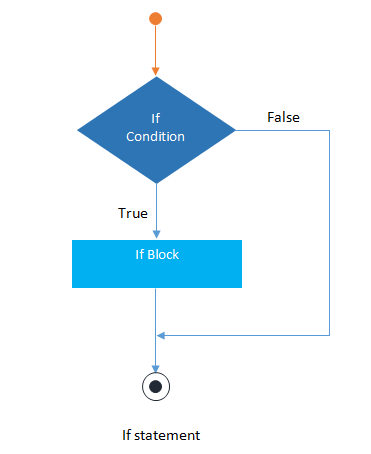
\includegraphics[width=0.2 \textwidth]{ifstatement.png}
		\label{Imagen_if}
	\end{SCfigure}
	
\underline{Dupla instrução condicional}
\\
\textbf{IF-ELSE}

\par{A declaração IF-ELSE estende a declaração se especificando uma ação se a se (expressão verdadeira/falsa)
é falsa.
Uma outra cláusula pode ser acrescentada a um simples condicional para especificar quais as linhas de código a executar, se a expressão booleana é falsa. Neste caso, estamos falando da estrutura se-senão, que no processo é expresso de acordo com este código [isc, ].}
\\
if (condição)\\
\{ \\
   fazer isto se a condição for verdadeira\\
   se declarações verdadeiras\\
\} \\
else \\
\{ \\
fazer isto se condição é falsa \\
se falsas declarações \\
\}
\par{Com a declaração se, um programa executará o verdadeiro bloco de código ou não fará nada. Com o se/senão o programa executará ou o bloco de código verdadeiro ou o bloco de código falso, portanto algo é sempre executado com uma declaração se/senão [isc, ].}
\begin{itemize}
    \item  Se a expressão for avaliada a não zero (verdadeiro), então a(s) declaração(ões) de bloco se for(em) executada(s).
    \item{Se a expressão for avaliada a zero (falsa), então a(s) declaração(ões) de bloco senão é(são) executada(s).}
\end{itemize}
\begin{SCfigure}[0.8][ht]
	    \centering
		\caption{If-else-ladder, (Obtained from: {DotNetTricks})}
		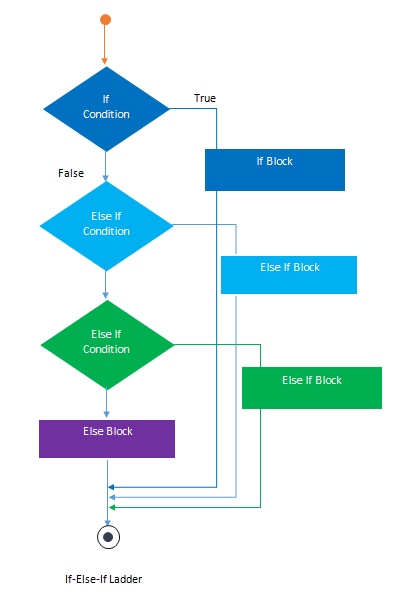
\includegraphics[width=0.2 \textwidth]{if-else-if ladder.png}
		\label{Imagen_If-else}
	\end{SCfigure}
	
\vspace{0.5 cm}
\underline{Declaração condicional múltipla}\\
\textbf{SWITCH}
\par{Permite a comparação de uma variável com diferentes valores possíveis, executando uma série de instruções específicas para cada caso. A declaração Switch atua como um substituto para uma longa escada se-senão-se que é utilizada para testar uma lista de casos. Uma declaração Switch contém uma ou mais etiquetas de casos que são testados contra a expressão. Quando a expressão corresponde a um caso, então as declarações associadas a esse caso seriam executadas.

\\
Escada if-else, mas a necessidade de uma forma adicional de lidar com as declarações condicionais pode parecer desnecessária, mas com base no uso específico, foi definido um caso de mudança para verificar a condição única, e com base nos múltiplos casos, o código pode ser executado.}
\vspace{0.5 cm}
Switch (expression) \{ \\
   valor da caixa 1: \\
     //  Declarações executadas quando o resultado da expressão
     corresponde ao valor 1
      [pausa;]
 
     
     \vspace{0.5 cm}
     
valor de caso 2:
// Declarações executadas quando o resultado da expressão
corresponde ao valor 2 [intervalo;] …
 \\
 
  valor da caixa, n:
// Declarações executadas quando o resultado da expressão
corresponde ao valor n [intervalo;]

   padrão: \\
     // Declarações executadas quando nenhum dos valores coincide com o valor da expressão
\vspace{0.5 cm}
     [pausa;] \\
\} \\

\begin{SCfigure}[1][ht]
	    \centering
		\caption{Switch statement, (Obtained from: {DotNetTricks})}
		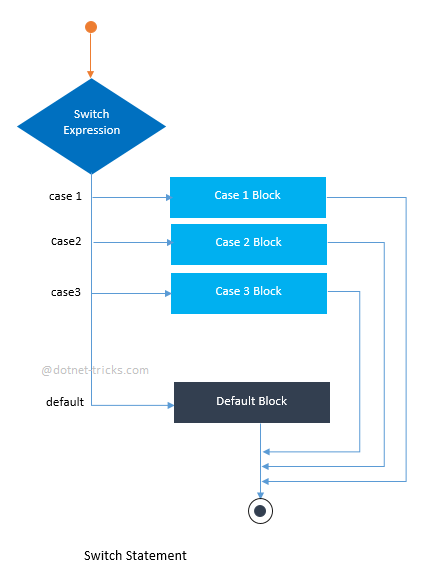
\includegraphics[width=0.5 \textwidth]{switch.png}
		\label{Imagen_Switch}
	\end{SCfigure}
	
\par{Algumas observações sobre esta estrutura:
\begin{itemize}
\item  É necessário pelo menos um caso.
\item Se vai utilizar poucos casos, talvez queira considerar a utilização de alguns se-senão em vez de switchcase.
\item A cláusula padrão é opcional. Não é obrigado a colocá-la, mas é aconselhável.
\item A quebra de declaração; impede o processamento de executar as seguintes linhas do caso seguinte.
\end{itemize}
\par{Por exemplo, se a primeira pausa não tivesse sido estabelecida no exemplo acima, então as mensagens "segunda-feira" e "terça-feira" seriam afixadas. O seguinte exemplo deve esclarecer este aspecto}}\\ \\
\textbf{WHILE}
\par{São utilizados quando queremos repetir a execução de declarações um número indefinido de vezes, uma vez que desde que uma condição seja cumprida. É mais fácil de compreender do que o loop FOR, uma vez que não incorpora a inicialização das variáveis, a sua condição para continuar a execução e a sua atualização na mesma linha.
Indica apenas, como veremos a seguir, a condição que deve ser preenchida para que uma iteração seja levada adiante}\\
   \begin{itemize}
       \item A condição será sempre avaliada antes de cada iteração.
       \item O corpo do loop do enquanto repete-se desde que a condição seja verdadeira.
       \item O corpo do loop do enquanto executa zero ou mais vezes.
   \end{itemize}
   \par{Uma expressão que é avaliada antes de cada etapa do laço. Se esta condição for avaliada como verdadeira, a declaração é executada. Quando a condição é avaliada como falsa, a execução continua com a declaração depois do loop while.} \\
   
   \begin{SCfigure}[1][ht]
	    \centering
		\caption{ Declaração While, ({DotNetTricks})}
		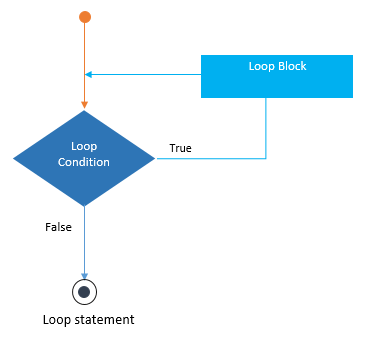
\includegraphics[width=0.2 \textwidth]{cloop.png}
		\label{Imagen_while}
	\end{SCfigure}
	\par{Normalmente,o loop While é útil quando não se tem conhecimento do número exato de iterações.}\\
	
    \underline{Declaração de controle repetitivo}\\
    \textbf{DO-WHILE}\\
    \par{É usado para executar um bloco de instruções pelo menos uma vez. O corpo do laço é repetido enquanto a condição é verificada. Esta condição será avaliada após cada repetição, usando uma das declarações do loop. Por exemplo, podemos imprimir números de 1 a 100 usando todos os loops.}\\ \\
    do\\
    \{ \\
    instrução 1 \\
    ... \\
    instrução n\\
    \} while (condition); \\
    \par{Normalmente, o laço para é útil quando você está ciente do número exato de iterações. Normalmente, ele é usado para iteração sobre matrizes e para processamento seqüencial.}
    
    \begin{itemize}
\item O corpo de um laço de faça-enquanto executa uma ou mais vezes.
\item O corpo do laço é repetido desde que a condição seja verdadeira.
\item A condição será sempre avaliada após cada iteração.
\end{itemize} \vspace{0.5 cm}
\textbf{For} \vspace{0.5 cm}
\par{É usado para executar um bloco de instruções um número fixo de vezes que é conhecido com antecedência. O laço para é mais conveniente com laços de contagem. Laços que são baseados em uma variável de contagem, geralmente um número conhecido de iterações. a instrução pode ser uma instrução única ou uma instrução composta (bloco), portanto, uma forma alternativa de escrever o formato pode ser:}\\

    for (initialCondition; testExpression;iterativeStatement)\\ 
 \{\\
    statement1;\\
    statement2;\\
    // ...\\
    statementN;\\
 \}\\
\par{Como funciona:\\
A condição inicial funciona uma vez, no início do laço A expressão de teste é verificada. (Isto é exatamente como a expressão em um laço enquanto). Se for falso, desista. Se for verdade,
\begin{itemize}
    \item Em seguida, executar o corpo do laço
    \item Execute a declaração iterativa
    \item Voltar à etapa de teste Expressão e repetir
\end{itemize}
}
    
  \newpage  
  


    
  

    
\newpage

\section{Exemplos de modelagem de sistemas biológicos no iGEM}
\par{Nesta seção, mostramos alguns exemplos de modelagem matemática de outros equipamentos no iGEM que pode servir como referência para modelar seu projeto. Convidamos você a visitar os wikis de outras equipes para que, como nós, você seja inspirado pelo incrível trabalho que outras equipes desenvolveram.}

    \subsection{Modelling a pathway that helps you decide which promoter to use.}
        \par{A equipe \href{https://2021.igem.org/Team:Vilnius-Lithuania/Model}{Vilnus-Lithuanian 2021 team} realizou uma modelagem matemática para escolher os pró-motores a modificar o caminho metabólico de seu organismo de uma maneira ideal.}
        \par{Eles começaram usando modelagem simples usando a cinética de Michaelis-Menten. Com isso, eles simularam a mudança do produto e do substrato de sua reação enzimática com relação ao tempo, Além disso, eles construíram equações diferenciais para modelar a concentração da enzima de interesse e suas respectivas mRNA.}
        \par{Finalmente, eles modelaram o caminho de síntese de Naringenin usando um sistema de equações químicas. Este foi convertido em equações diferenciais. E, com as suposições que fizeram, eles foram capazes de simplificar o modelo para algumas equações.}
        
        \begin{SCfigure}[0.65][h]
	    \centering
		\caption{caminho de síntese de Naringenin}
		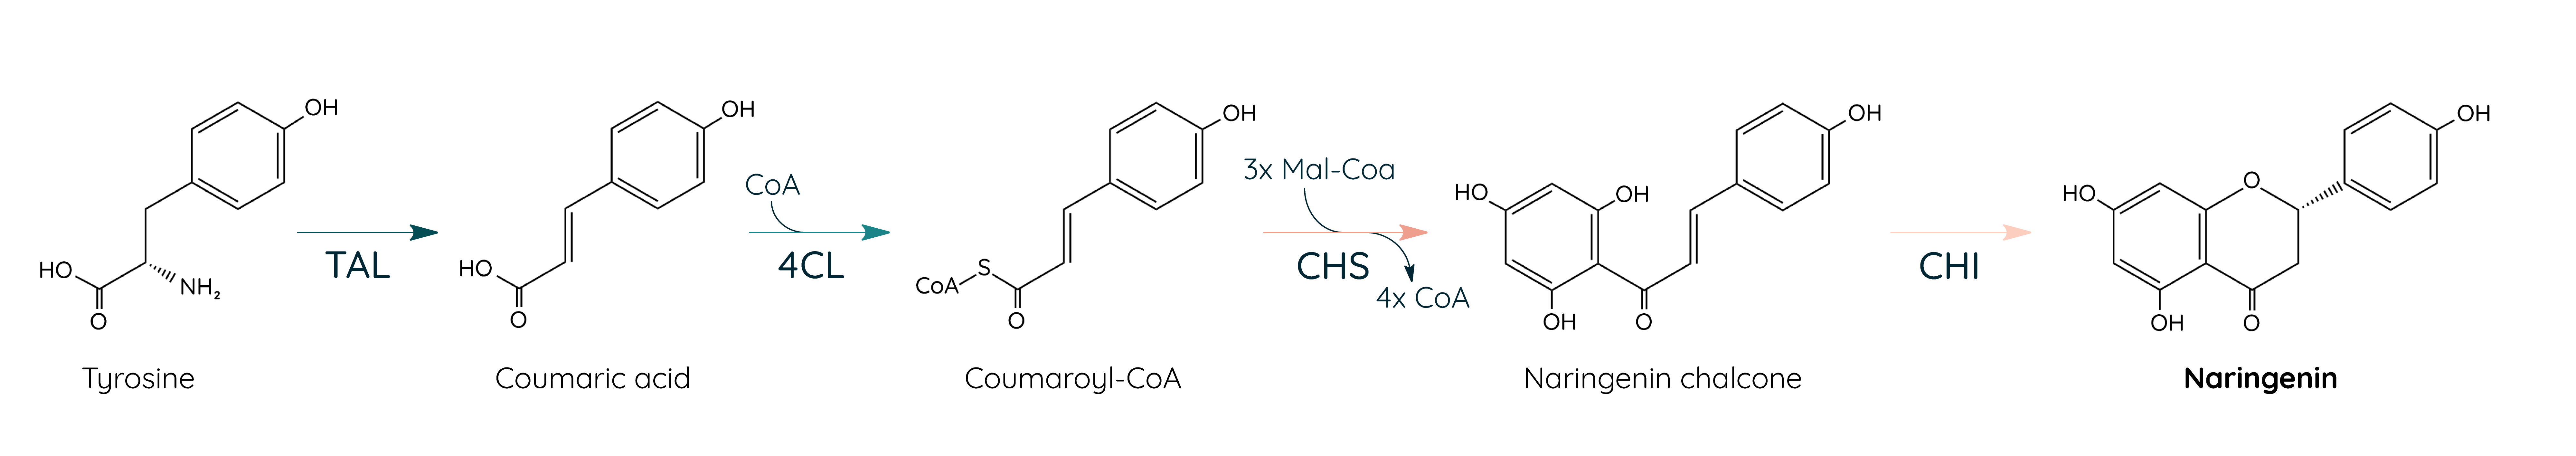
\includegraphics[width=0.65\textwidth]{Vilnus.png}
	\end{SCfigure}
	
\par{O modelo os ajudou a decidir qual promotor usar, e eles foram capazes de determinar a etapa de estrangulamento no caminho de síntese de Naringenin.}

\subsection{Modelagem do tempo necessário para produzir um componente de 
interesse
}
\par {Modelar a expressão gênica com um sistema de EDOs é uma tarefa muito comum nos projetos iGEM. Um bom exemplo disso é o trabalho realizado pelo \href{https://2015.igem.org/Team:Oxford/Modeling#characterising-our-cells}{iGEM Oxford} em 2015. Eles trabalharam em um projeto que foi concentrado em fazer uma alternativa aos antibióticos para o tratamento de infecções urinárias. Para isso, eles projetaram a \textit{Escherichia coli} para produzir enzimas que poderiam quebrar os biofilmes bacterianos responsáveis pela geração de infecções urinárias. Naturalmente, era necessário saber se suas bactérias artificiais tinham a capacidade de produzir a quantidade necessária de enzimas. Esta é a parte em que a modelagem matemática entra.}

\par {Através de um sistema de EDOs, a equipe foi capaz de prever o tempo necessário para produzir uma quantidade de suas proteínas de interesse. Usando um sistema de expressão induzida por arabinoses, eles usaram a cinética de Michaelis Menten para gerar seu sistema e comparar seus resultados com dados experimentais para se adequar aos seus dados. Com estes, eles puderam calcular as concentrações limite de seus produtos. Um notável aspecto sobre este trabalho é a consideração e pesquisa de seus parâmetros de modelo, o que dá grande validade para seu modelo \cite{iGEMOxford_2015}.}

\begin{SCfigure}[0.65][ht]
	    \centering
		\caption{Parâmetros bem documentados validam o modelo de uma equipe e ajudam as equipes futuras a construir seus próprios sistemas \cite{iGEMOxford_2015}}
		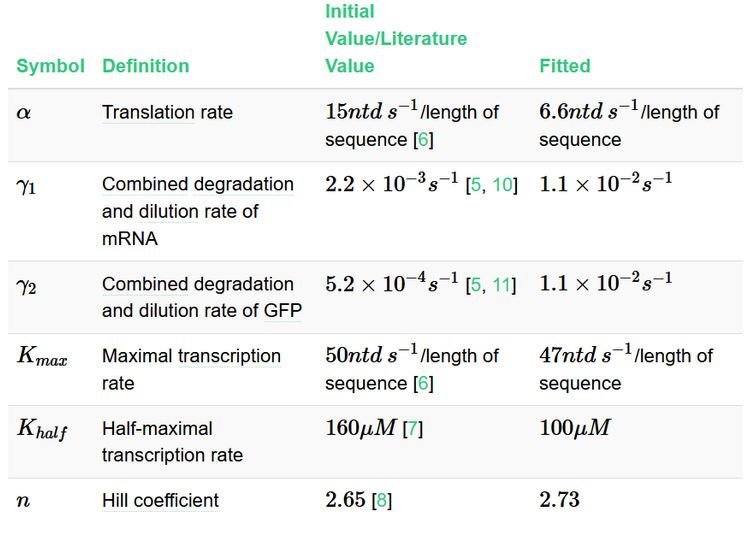
\includegraphics[width=0.65\textwidth]{Tabla parametros.JPG}
	\end{SCfigure}
	\vspace{0.3 cm}
	
    \subsection{Modelagem de uma reação de Michaelis-Menten\texorpdfstring{$-$}{Lg}Reação de Menten}
    \par {Outro exemplo é o modelo da equipe do \href{https://2018.igem.org/Team:Queens_Canada/Michaelis-Menten_Kinetics}{Queens Canada 2018 team.} Eles fizeram vários processos de modelagem, mas vamos nos concentrar na seção Cinética de Michaelis-Menten que ajuda na análise da cinética enzimática.} 
    \par {Nesta parte eles fizeram uma calculadora que funciona com as entradas de concentração do substrato, produto concentração e concentração enzimática, essas informações são colocadas em uma função que gera a taxa de mudança de concentração. Este programa foi feito no MATLAB e eles colocaram o código em sua wiki, assim outras equipes podem usar a calculadora no futuro.}
    
    \subsection{Modelagem da produção, do mecanismo de entrega e do silenciamento das moléculas iRNAs}
\par{Para a América Latina, a agricultura é uma fonte de trabalho e renda para milhões de pessoas. O Equador é um dos principais países país na exportação e produção de bananas, isto estava em risco devido a uma doença, a murchidão. Por isso, a equipe do iGEM Equador 2021 desenvolveu a AgroBactory 593, uma plataforma de célula bacteriana modular que fabrica biopesticidas usando a tecnologia RNAi para combater doenças nas plantas, como a murcha causada por \textit{Fusarium oxysporum f. sp. cubense} (Foc R4T) em
bananas. O meio de entrega para isto foi planejado a ser feito por injeção direta do dsRNA no tronco e também por uma bactéria vegetal que libera o dsRNA através de um sistema oscilatório de lise.}
\par{Seu modelo dinâmico explicou a inibição dos ingredientes ativos do Agrobactory com EDOs e dois sistemas de expressão, um de dsRNA e outro do promotor T7 e IPTG para expressão dsRNA. Isto seria dividido em três seções:}
\begin{enumerate}
            \item \textbf{Produção de dsRNA} utilizando um promotor constitutivo, as células Agrobactory produzem dsRNA a partir do gene alvo.
            \item \textbf{Entrega e liberação de moléculas de dsRNA} através de uma proteína de lise celular, ativada pelo quorum mecanismo de sensoriamento que aciona a lise celular.
            \item \textbf{O silenciamento do RNA} do gene Velvet e como as moléculas interferentes de dsRNA e RNA podem inibir sua expressão gênica e controlar a murcha causada por \textit{Fusarium}.
\end{enumerate}
\par{Este modelo explica claramente que tipo de modelo é e que informações serão obtidas graças a ele. Também menciona os parâmetros que foram utilizados, seus ajustes e são referenciados. Este ajudou a equipe a entender como funcionava seu sistema de expressão, e os mecanismos de entrega e de silenciamento, e usaram as medidas para entender, desenvolver e melhorar o modelo.}
\par{O modelo é impressionante porque permite conhecer a produção, o mecanismo de entrega e o silenciamento do dsRNA da Agrobactory, eles também utilizaram diagramas que facilitam sua compreensão e simulações computacionais que provam que a Agrobactory é funcional. Que podem ser usadas para fazer futuras previsões e é de grande ajuda para outras equipes que estão realizando projetos similares.}

\newpage

\section{Resumo dos programas e modelos}
\par{As ferramentas bioinformáticas podem ser muito úteis, você pode ter uma ideia muito boa do que você está procurando, como suas estruturas em 3D, a ligação entre as proteínas, as sequências, como sua construção vai trabalhar, modelagem de construções biológicas, e muitas outras características. Tudo isso é essencial quando você está trabalhando em modelagem matemática, porque esta informação pode facilitar as coisas quando se trabalha no laboratório.
}
\subsection{Ferramentas de computador para modelagem}
\par{Para construir um modelo matemático, precisamos selecionar a estrutura de equações diferenciais, que transformar-se em um sistema que, com muitas incógnitas, emprega métodos numéricos. Para fazer isso, usamos programação:}

\begin{table}[h]
\begin{tabular}{| m{3cm} | m{9cm}|}
\hline
\multicolumn{1}{|c|}{\textbf{Programming Languages}}                                                                                                           \\ \hline
C & Os grandes programas são divididos em pequenos programas chamados funções que se concentram em funções e processos que operam com dados. \\ \hline
\multicolumn{1}{|l|}{C\#} &
  Uma linguagem de programação multiparadigma com fortes disciplinas de programação por escrito, imperativa, declarativa, funcional e orientada a objetos. \\ \hline
\multicolumn{1}{|l|}{C++}    & Uma extensão da linguagem C, mas de nível médio e orientada a objetos.                                                  \\ \hline
\multicolumn{1}{|l|}{Python} & Uma linguagem que é interpretada, orientada a objetos, e construída sobre uma semântica flexível e robusta.                                    \\ \hline
\multicolumn{1}{|l|}{Ruby}   & Uma linguagem de script de código aberto orientada a objetos que pode ser usada isoladamente ou como parte da estrutura web Ruby on Rails   \\ \hline
\multicolumn{1}{|l|}{PHP}    & Uma linguagem de script de código aberto projetada para criar páginas web dinâmicas que funcionam efetivamente com bancos de dados.                    \\ \hline
\multicolumn{1}{|l|}{Java}   & Uma linguagem de programação de alto nível e orientada ao usuário, ideal para o desenvolvimento baseado na web.                                              \\ \hline
\multicolumn{1}{|l|}{JavaScript} &
  Uma linguagem de programação do lado do cliente que roda dentro de um navegador do cliente e processa comandos em um computador em vez de um servidor. \\ \hline
\end{tabular}
\end{table}


\subsection{Models to use}
\par{Os modelos matemáticos podem ser classificados de acordo com várias características. Há um grande número de classificação diferente para modelos matemáticos. Entretanto, aqui resumimos alguns deles, seu propósito e um exemplo de uma equipe iGEM que os utilizou.} 

\begin{table}[h]

\begin{tabular}{ | m{3cm} | m{7cm}| m{6.2cm} | } 
\hline
\textbf{Tipo de Modelo} & {\color[HTML]{000000} \textbf{Breve descrição}}                                                                                                    & \multicolumn{1}{c|}{\textbf{Exemplo}}                                  \\ \hline
Determinístico                                 & Cada valor de parâmetro pode ser representado
como um número concreto
                                                                                        & A Equipe TuDelft iGEM 2021 utiliza um modelo determinístico para representar o rede biomolecular da AptaVita
(seu projeto)
 \\ \hline
Estocástico                                    & Cada parâmetro pode ser representado como um definido por valores aleatórios definidos com distribuições de probabilidade.
                                                  & Thessaly 2021 iGEM Team, utiliza ambos (determinístico e estocástico modelo) para simular seu projeto em silico.
             \\ \hline
Método Monte Carlo

                            & Esta é uma técnica matemática usada para o possíveis resultados de um evento incerto
                                                             &   Avaliar o impacto do risco sobre o estoque preço.
 %https://www.ibm.com/es-es/cloud/learn/monte-carlo-simulation                                                                                                                      
 \\ \hline
Otimização                                  & Este tipo de modelo é usado para encontrar os melhores parâmetros do objeto de estudo
                                                                    & Para encontrar a menor massa possível de um foguete lançado de algum lugar para alcançar uma parte exata do espaço.
            \\ \hline
Caótico                                       & Este modelo utiliza idéias da teoria do caos
para tratar de questões comuns durante o trabalho
em um ambiente de equipe. É geralmente usado como
uma metodologia de programação.
 & Como a poluição da Cidade do México influencia o turismo na cidade.                                                             \\ \hline
Complexo                                       & Os elementos do sistema e o próprio sistema interagem com os elementos do mundo ao redor, e estas interações pode mudar com o tempo.   & Modelar o trânsito de uma cidade.                                                                                         \\ \hline
    
\end{tabular}
\end{table}
\subsection{Declarações de controle}
\par{Os três tipos de condicionadores (simples, duplos e múltiplos) permitem que o programa execute certas linhas de código quando uma condição é cumprida, desde que uma condição seja cumprida. Para resumir, as declarações de controle são as seguintes:}

\begin{center}
\begin{tabular}{ | m{3cm} | m{4cm}| m{9.2cm} | } 
\hline
Declarações & Tipo de condicional & Função \\\hline
If (Se) & Simples & Executar linhas de código se uma condição for cumprida \\\hline
Else (Senão) & Simples & Cláusula acrescentada a uma simples condicional para executar linhas de código se uma condição não for cumprida
 \\\hline
Switch & Dupla & Compara uma variável com valores possíveis e executa
a que é cumprida
 \\\hline
While (Enquanto) & Dupla & Repeats a Repete uma declaração desde que uma condição seja cumprida \\\hline
Enquanto & Repetitivo & Executa uma declaração pelo menos uma vez e a repete desde que uma condição seja cumprida \\\hline
For (Para) & Repetitiva & Executa código um número fixo de vezes\\\hline
\end{tabular}
\end{center}


\newpage 

\bibliographystyle{apalike}
\bibliography{ref}

\end{document}